\subsection{Sơ đồ hoạt động}
% --- PHẦN 1: XÁC THỰC VÀ TÀI KHOẢN (AUTHENTICATION & ACCOUNT) ---

\begin{figure}[H]
    \centering
    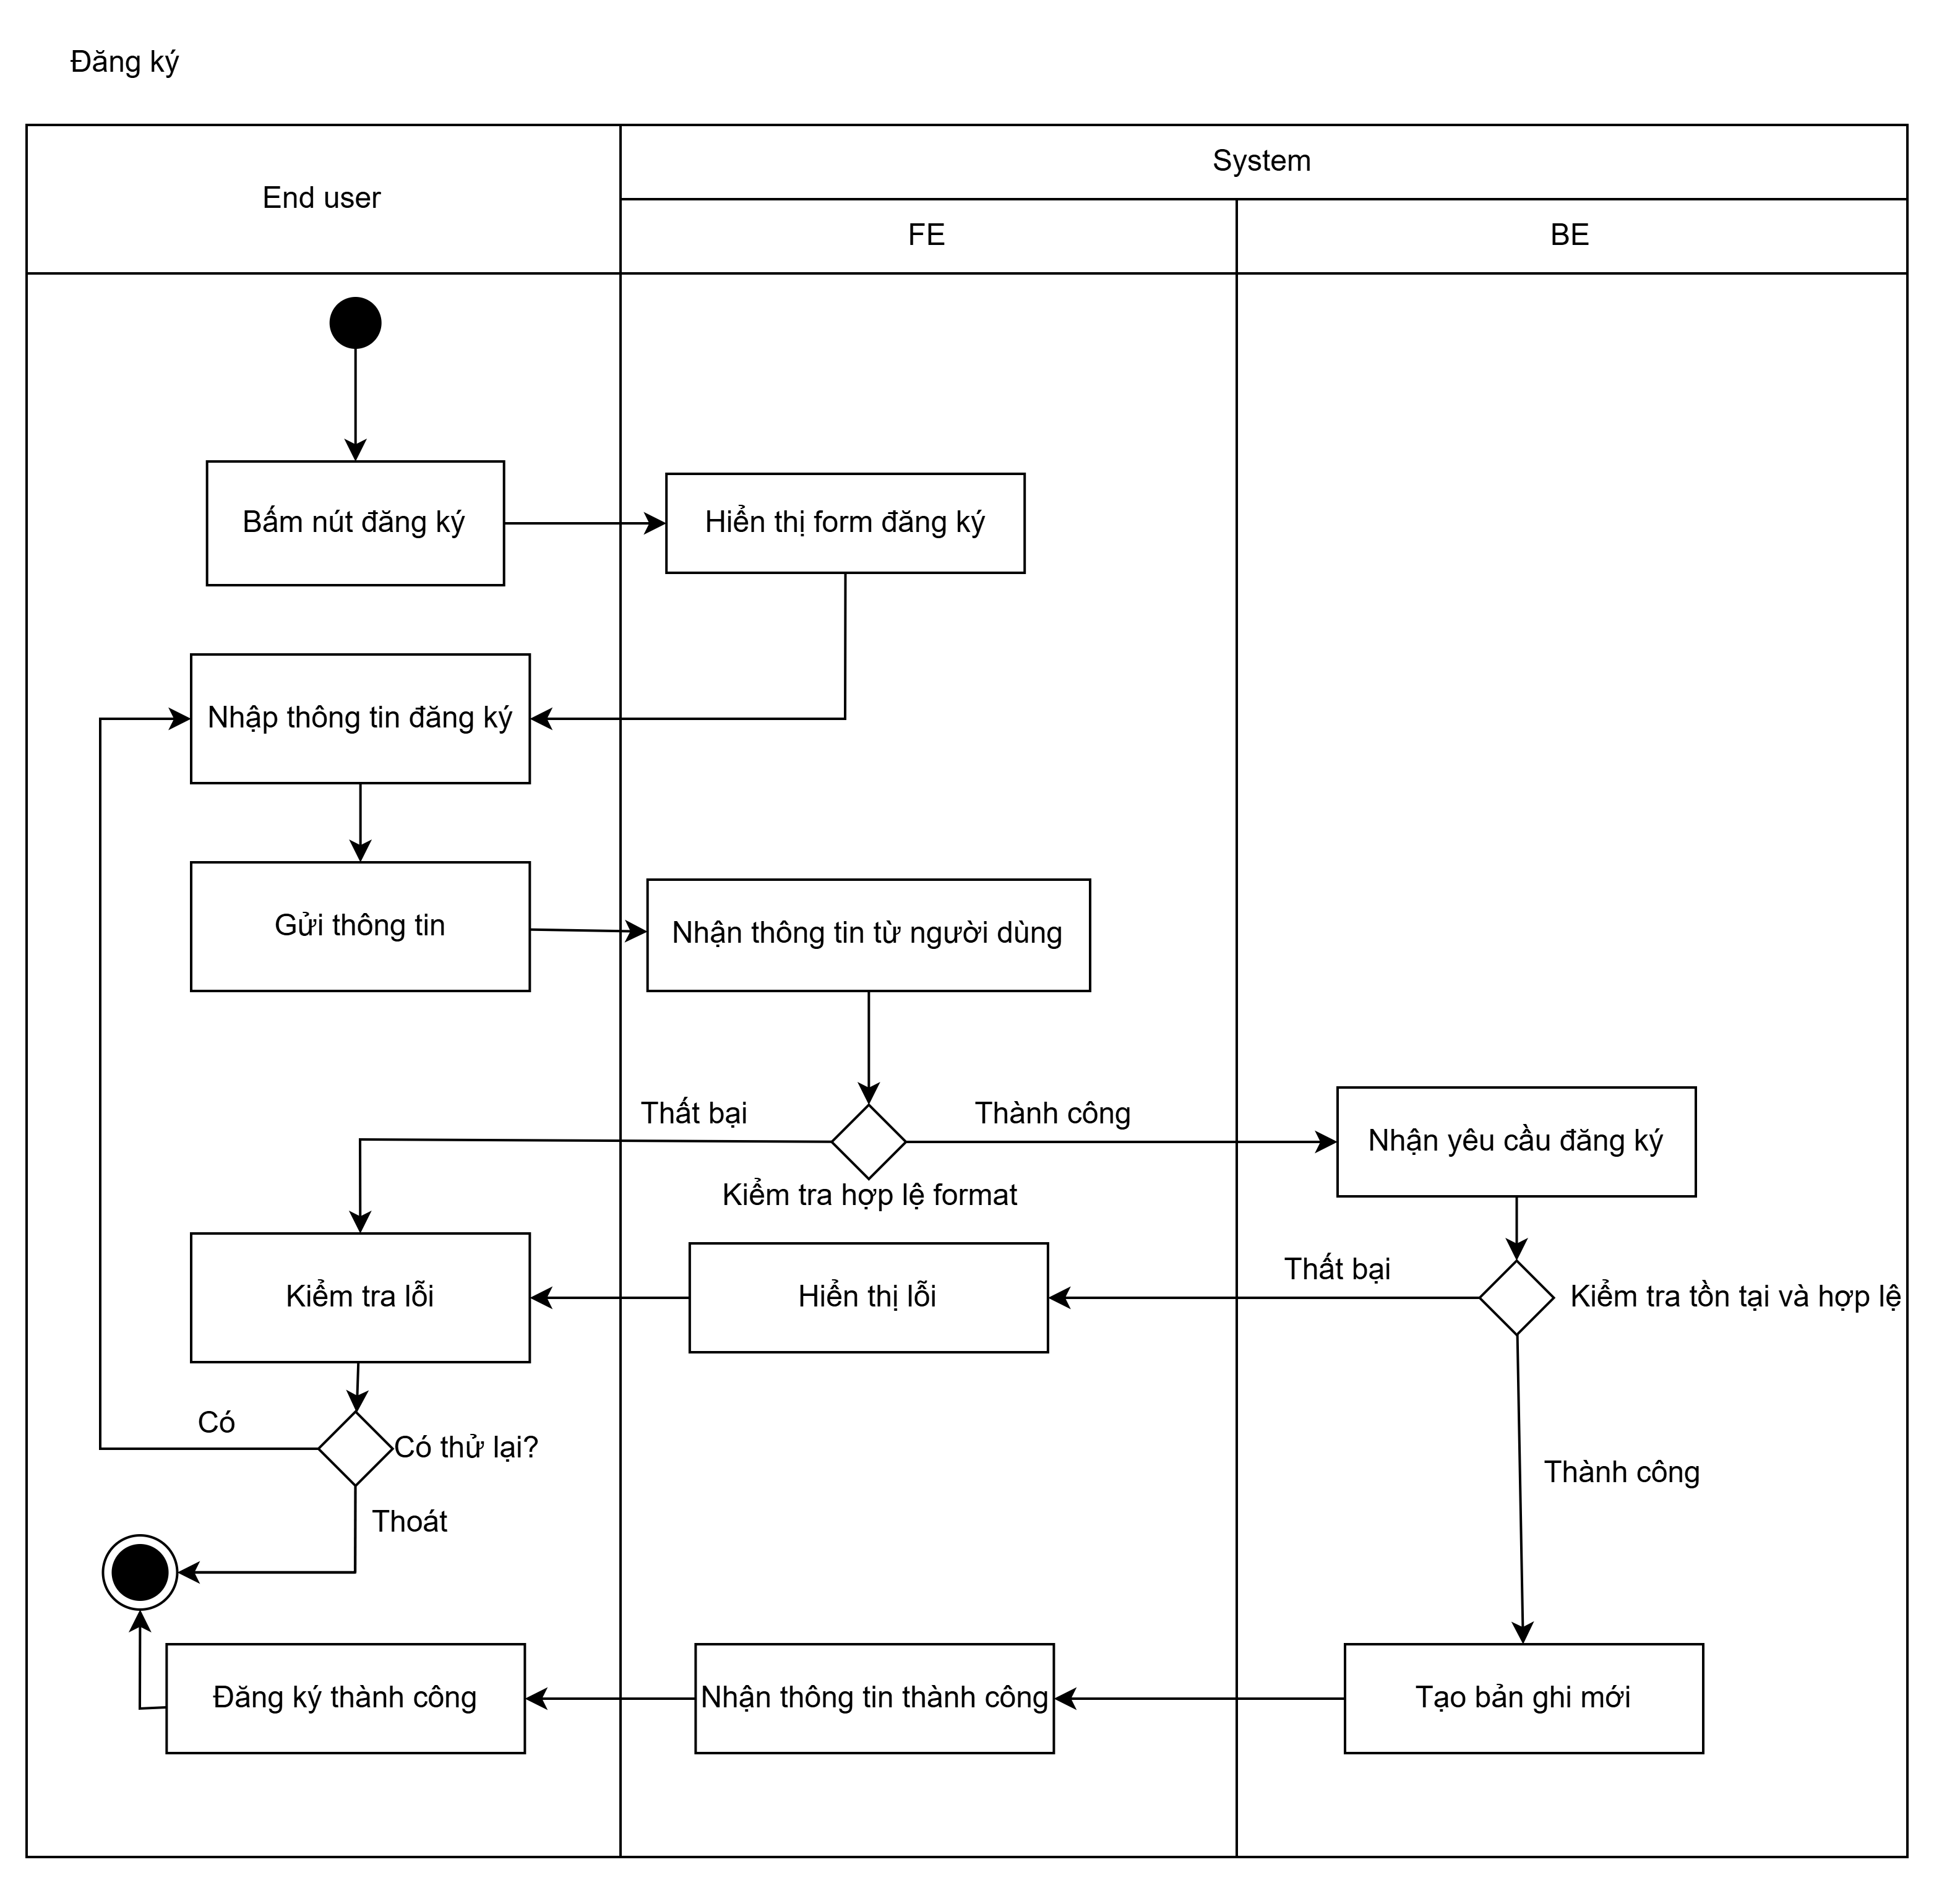
\includegraphics[width=0.7\linewidth]{images/chap3/activity_diagram/register.png}
   \vspace{0.5cm} 
   \caption{Sơ đồ hoạt động chức năng Đăng ký tài khoản}
    \label{fig:act_register}
\end{figure}
Mô tả quy trình người dùng mới nhập thông tin cá nhân. Hệ thống kiểm tra tính hợp lệ của dữ liệu (email, mật khẩu), tạo tài khoản mới trong cơ sở dữ liệu và thông báo kết quả đăng ký.

\begin{figure}[H]
    \centering
    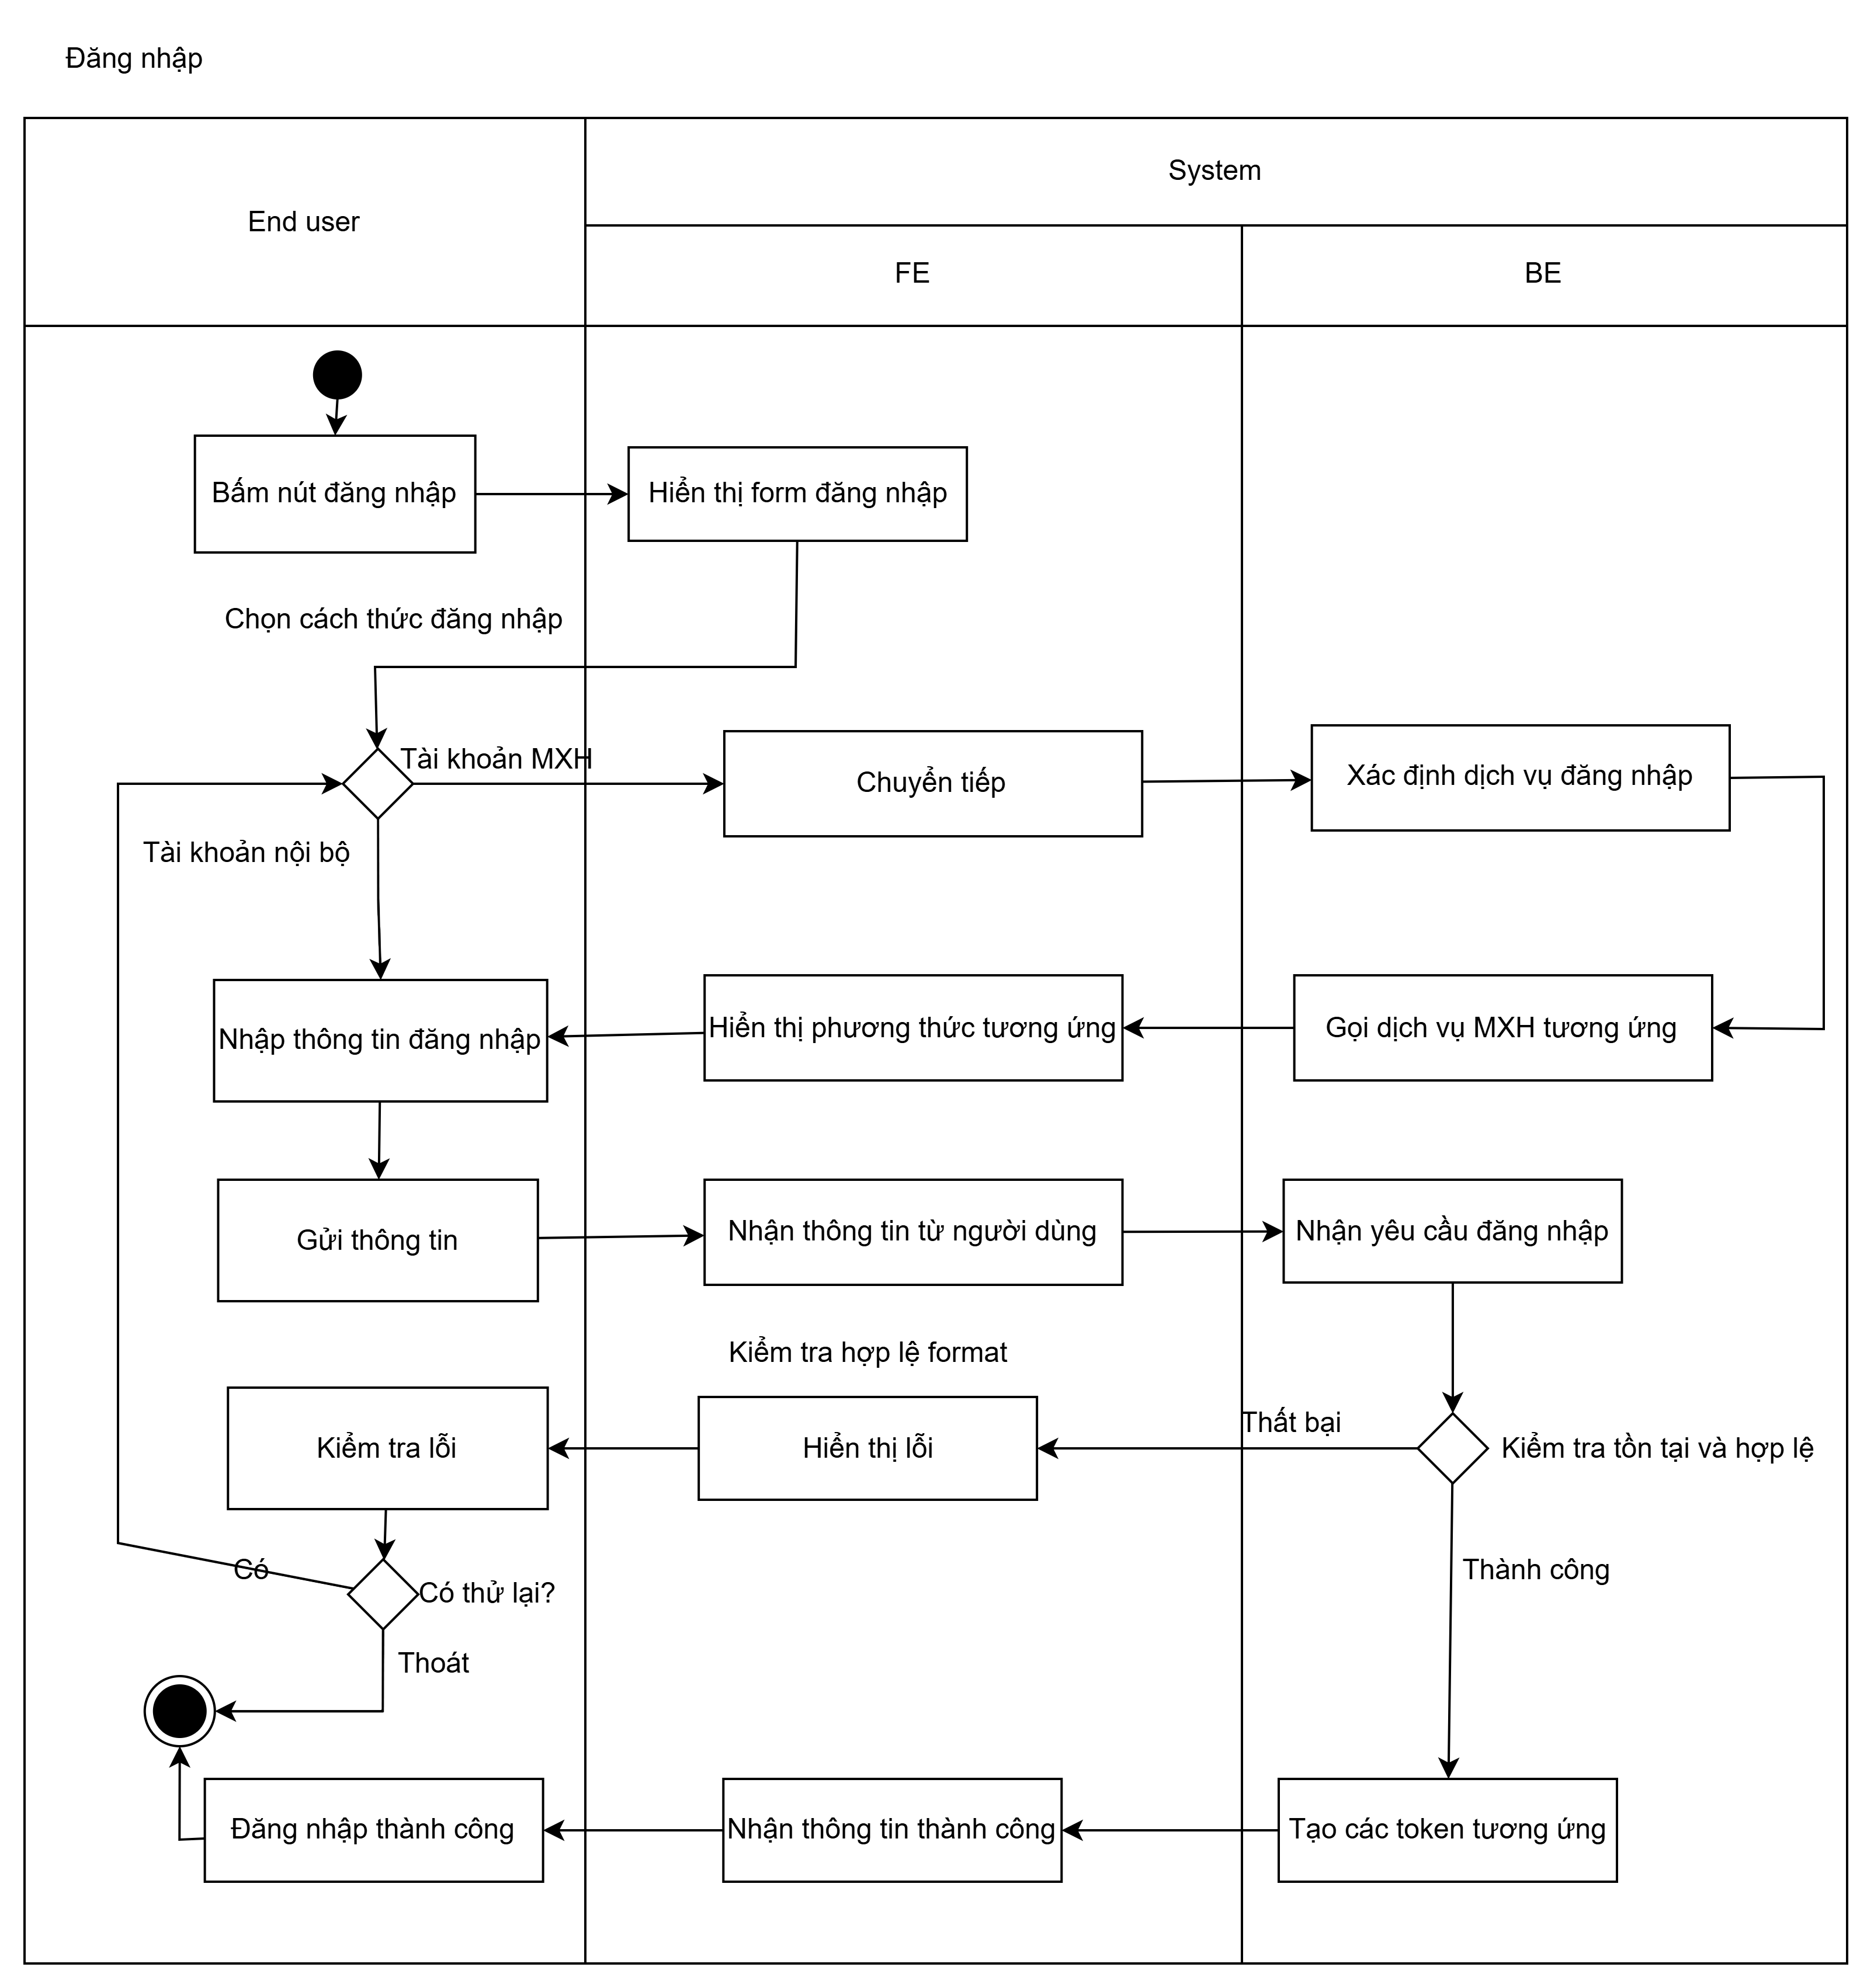
\includegraphics[width=0.7\linewidth]{images/chap3/activity_diagram/login.png}
   \vspace{0.5cm} \caption{Sơ đồ hoạt động chức năng Đăng nhập}
    \label{fig:act_login}
\end{figure}
Mô tả quá trình người dùng nhập thông tin xác thực. Hệ thống đối chiếu với cơ sở dữ liệu, cấp quyền truy cập (token/session) nếu thông tin đúng hoặc báo lỗi nếu sai lệch.

\begin{figure}[H]
    \centering
    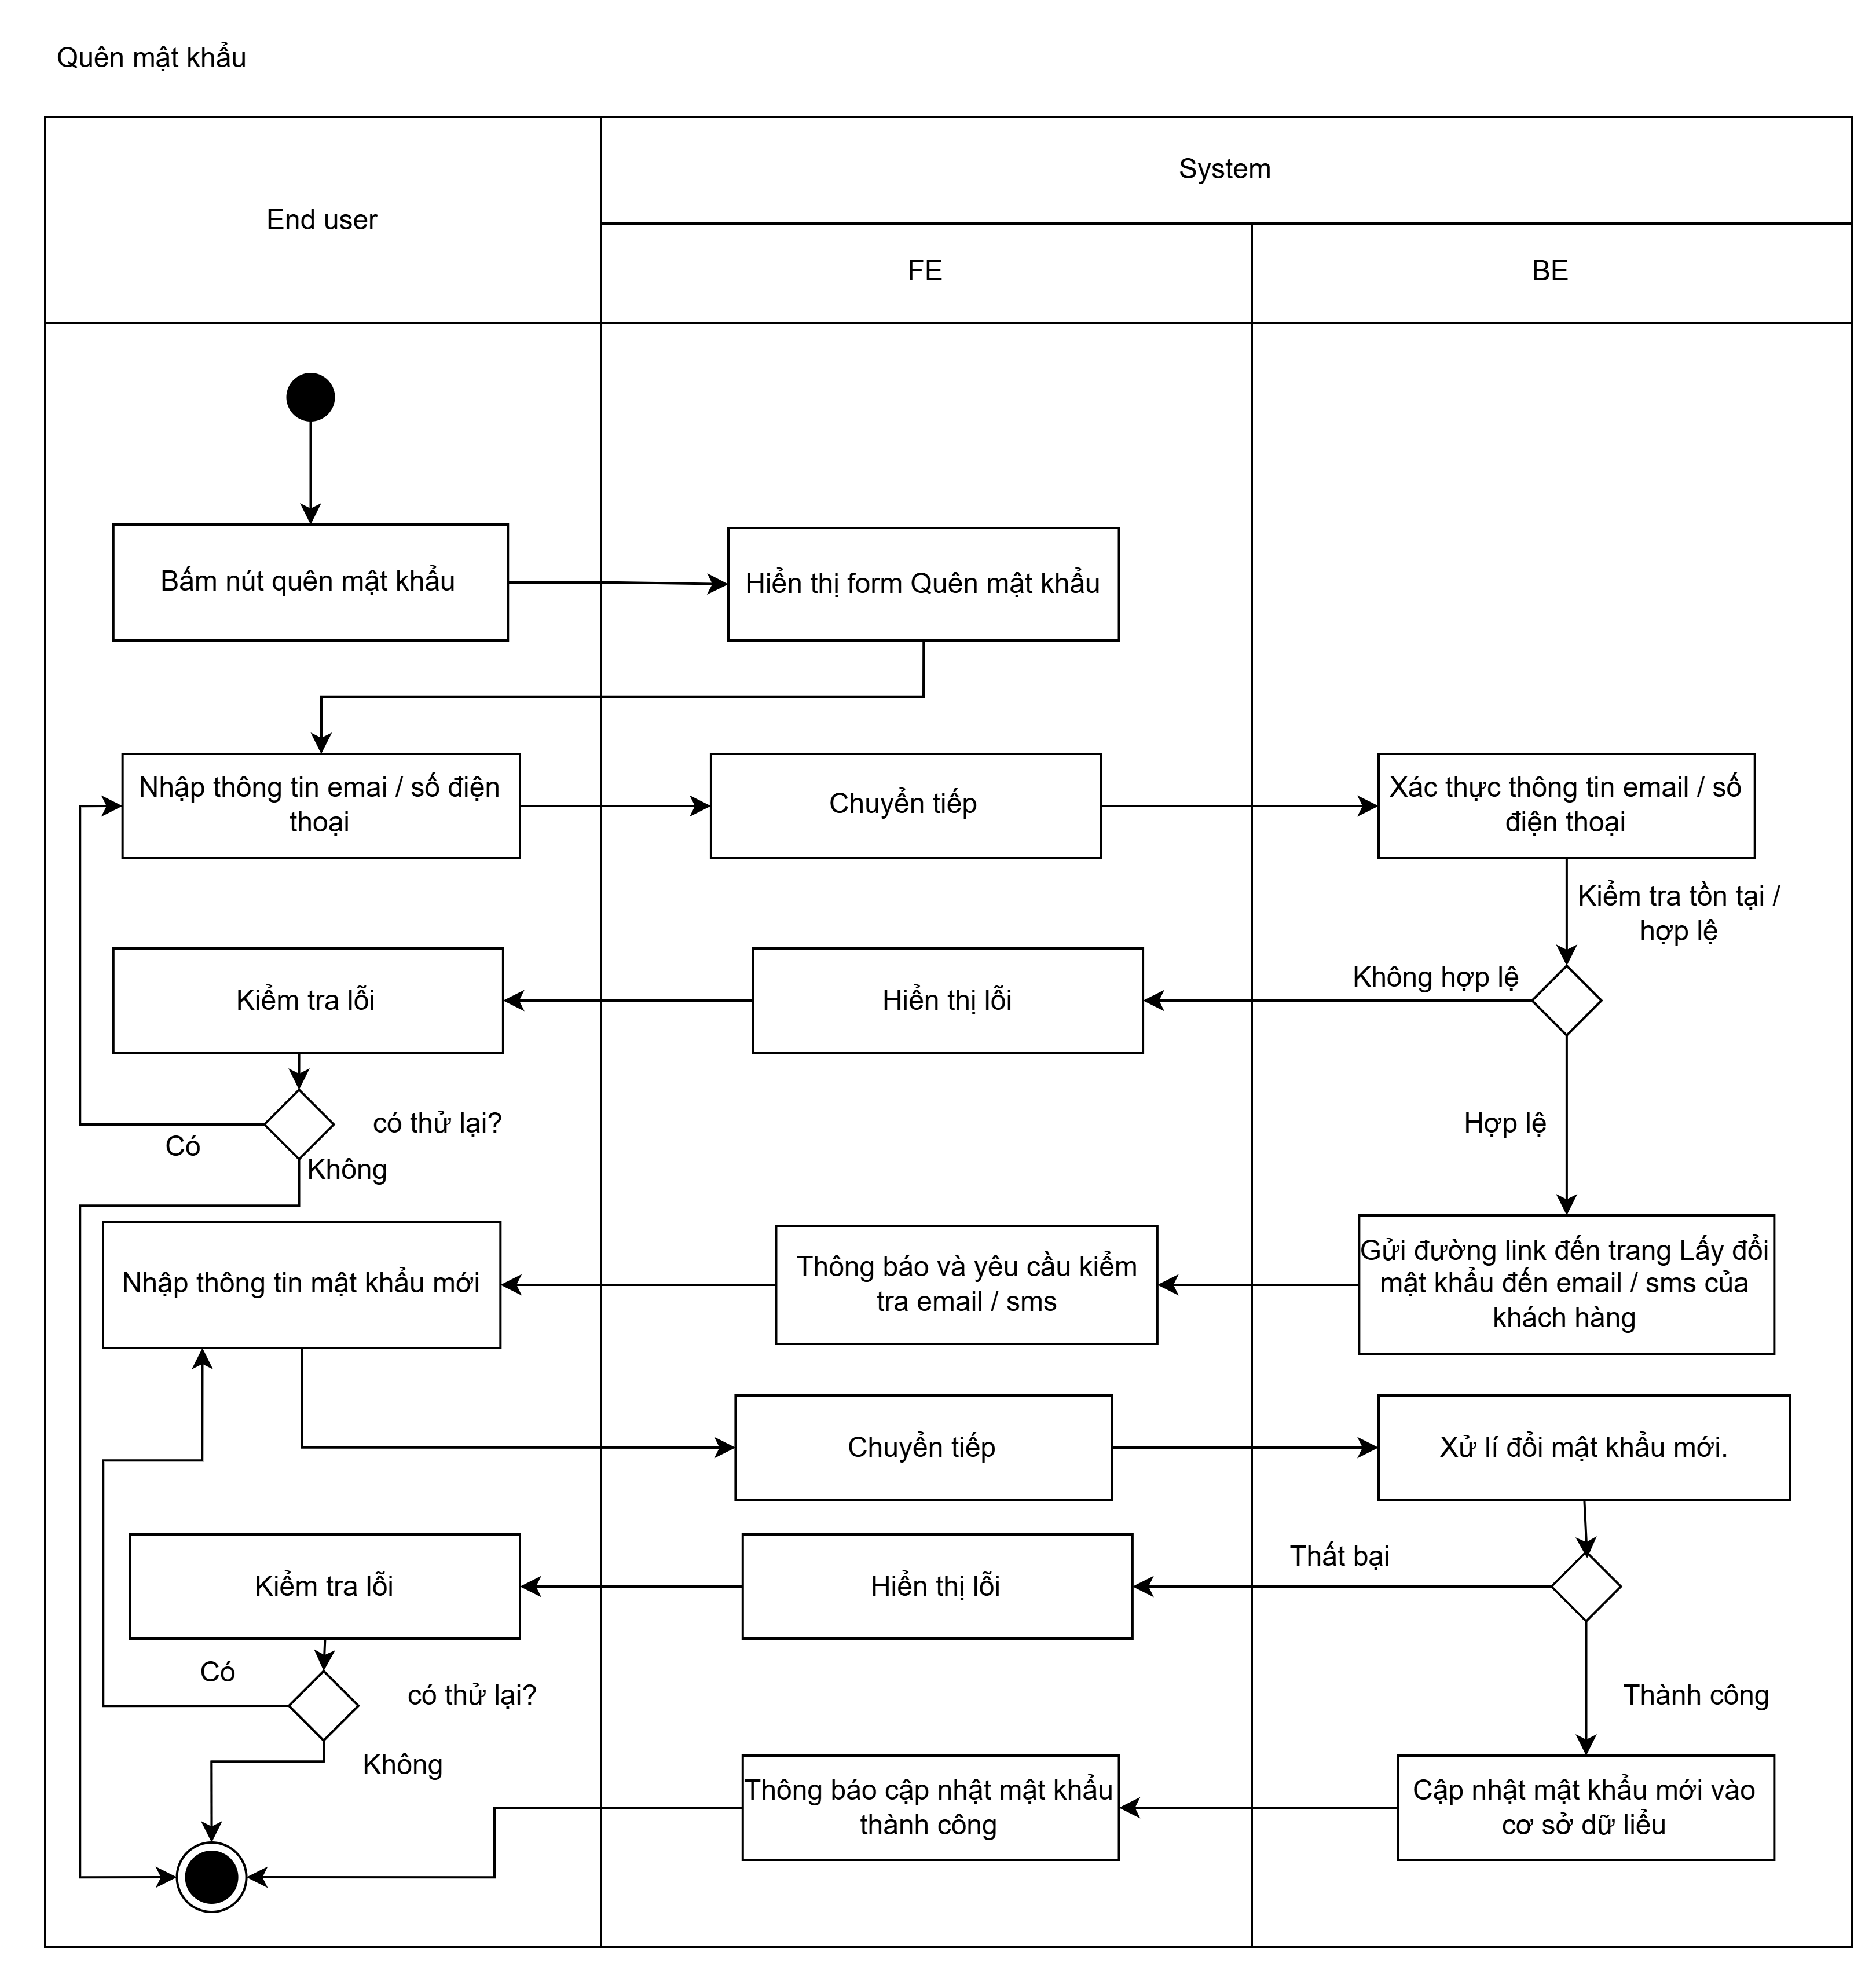
\includegraphics[width=0.7\linewidth]{images/chap3/activity_diagram/forgot_password.png}
   \vspace{0.5cm} \caption{Sơ đồ hoạt động chức năng Quên mật khẩu}
    \label{fig:act_forgot_pass}
\end{figure}
Mô tả quy trình khôi phục quyền truy cập khi người dùng quên mật khẩu, bao gồm các bước nhập email, xác thực mã OTP/Link và thiết lập mật khẩu mới.

\begin{figure}[H]
    \centering
    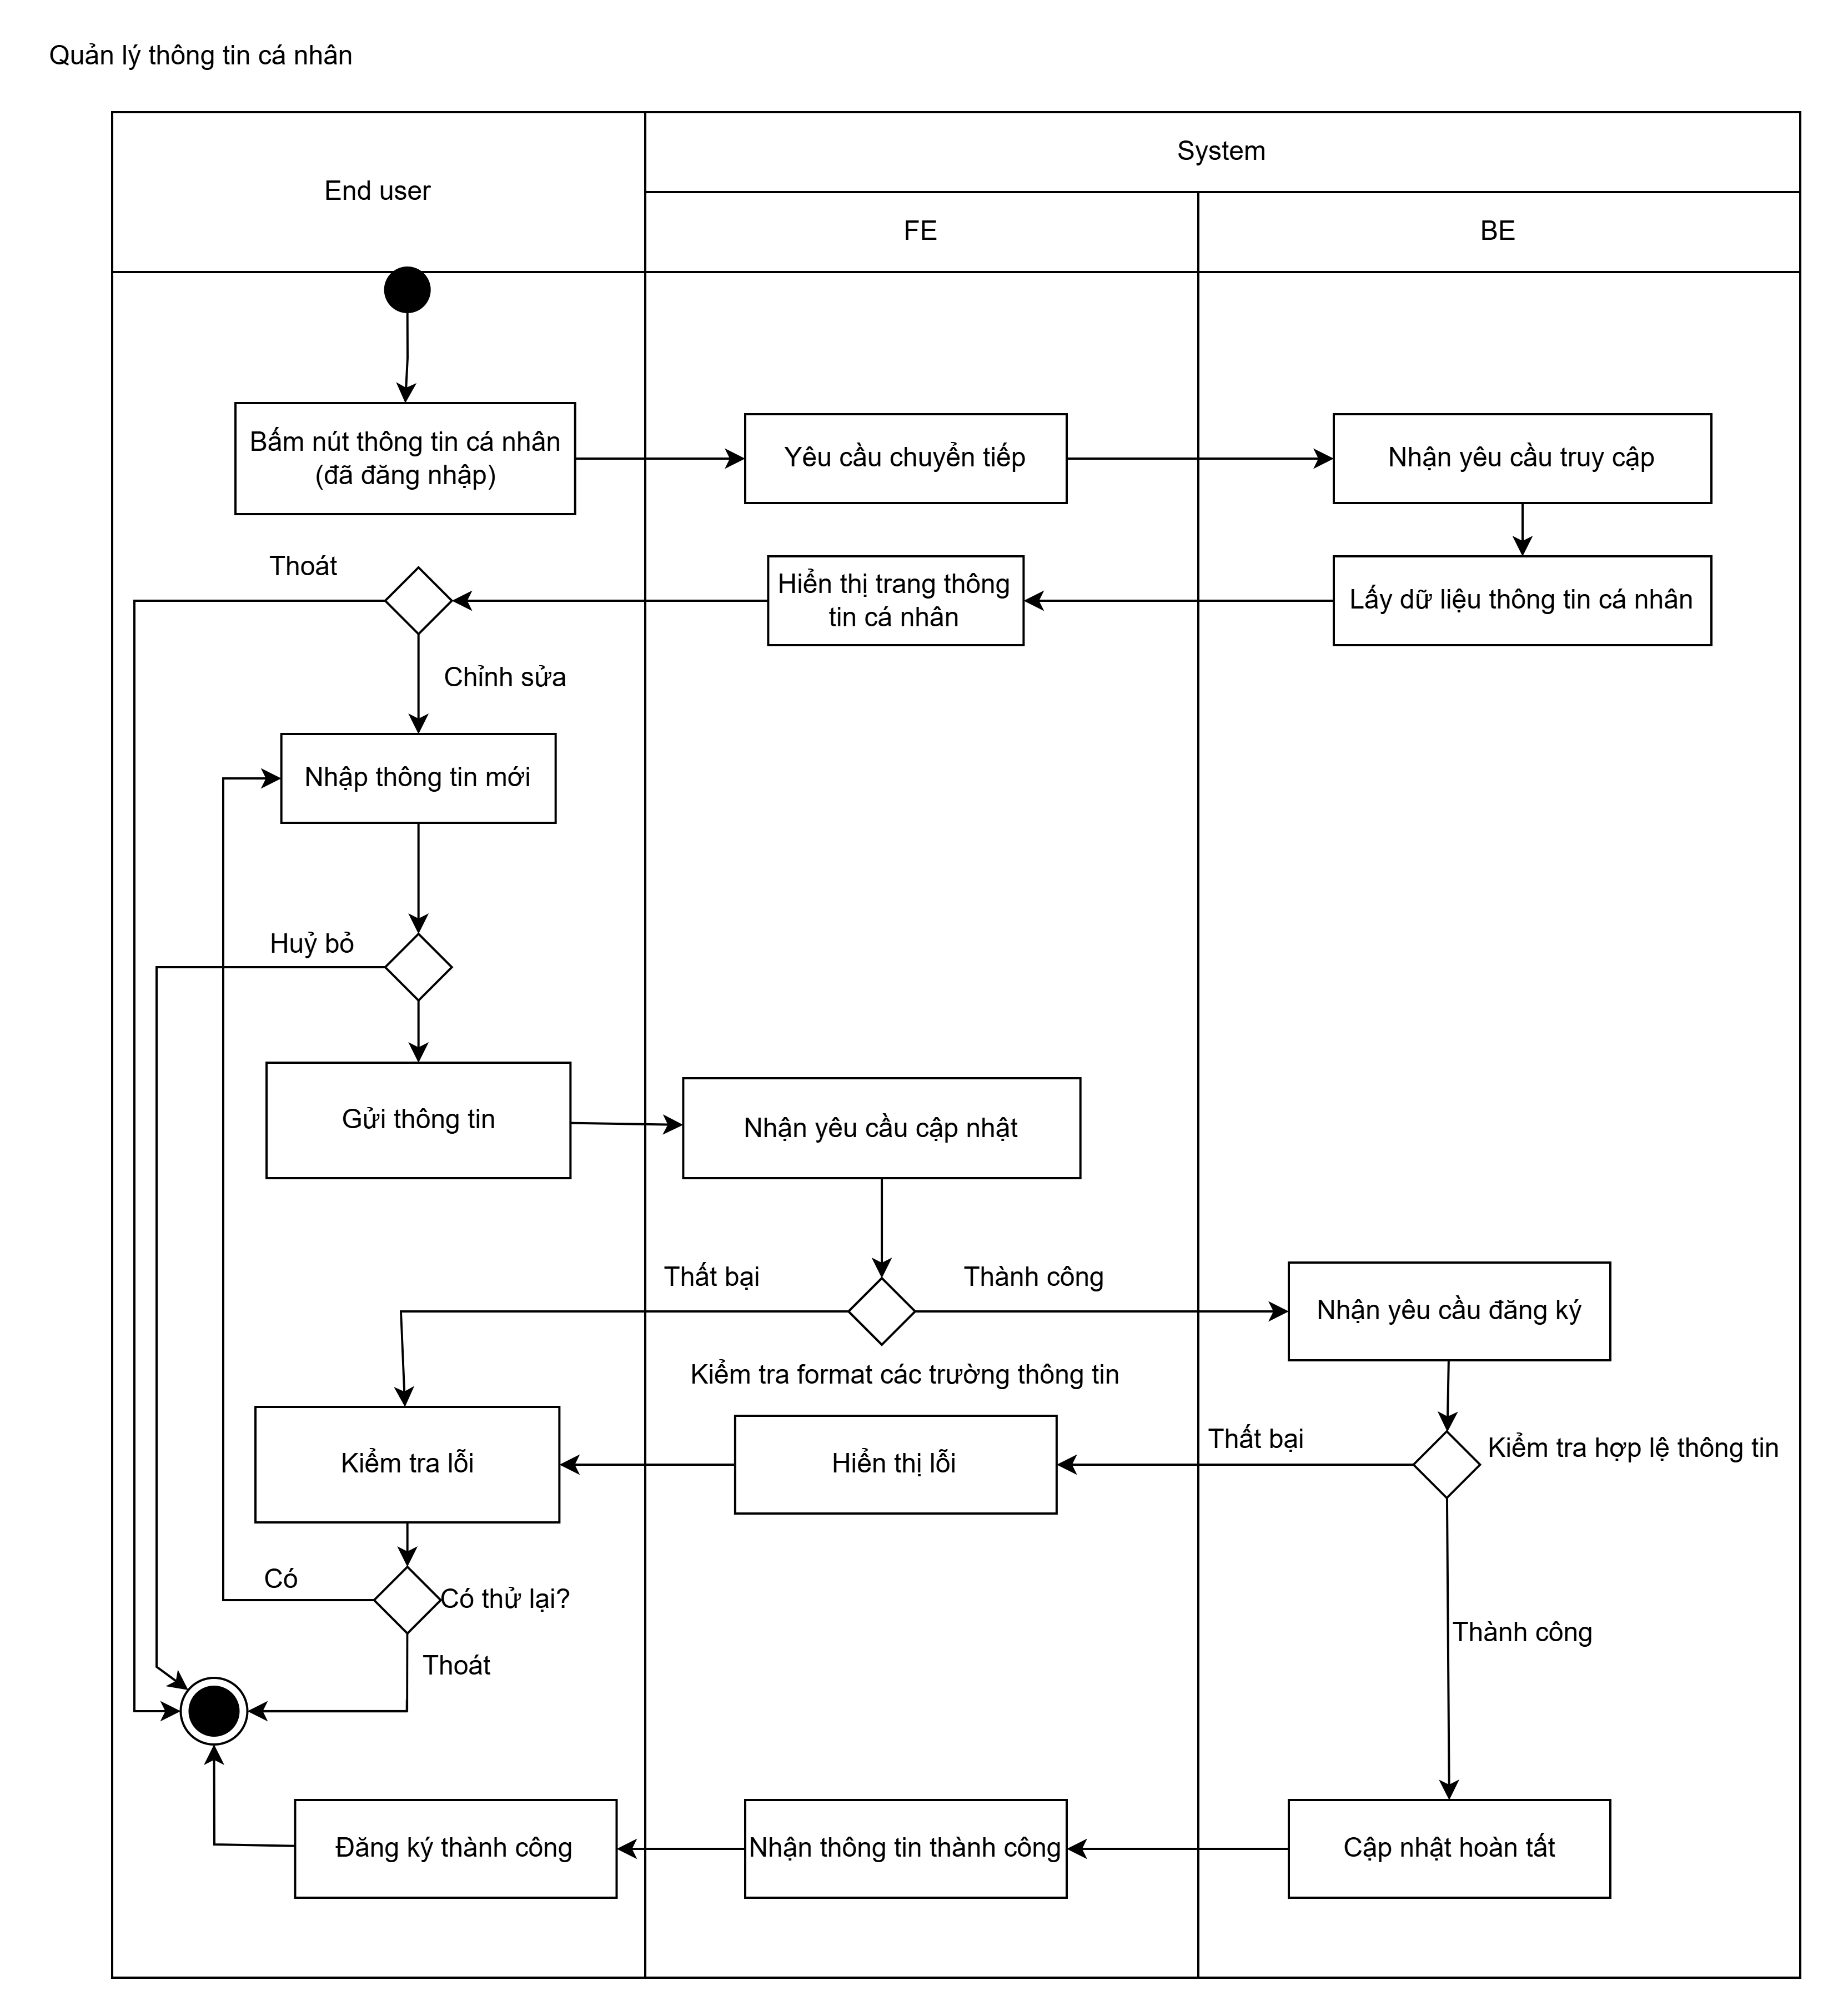
\includegraphics[width=0.7\linewidth]{images/chap3/activity_diagram/manage_personal_information.png}
   \vspace{0.5cm} \caption{Sơ đồ hoạt động Quản lý thông tin cá nhân}
    \label{fig:act_manage_info}
\end{figure}
Cho phép người dùng xem và chỉnh sửa thông tin hồ sơ cá nhân (tên, số điện thoại, địa chỉ), sau đó cập nhật lại vào hệ thống.

% --- PHẦN 2: MUA SẮM VÀ THANH TOÁN (SHOPPING & PAYMENT) ---

\begin{figure}[H]
    \centering
    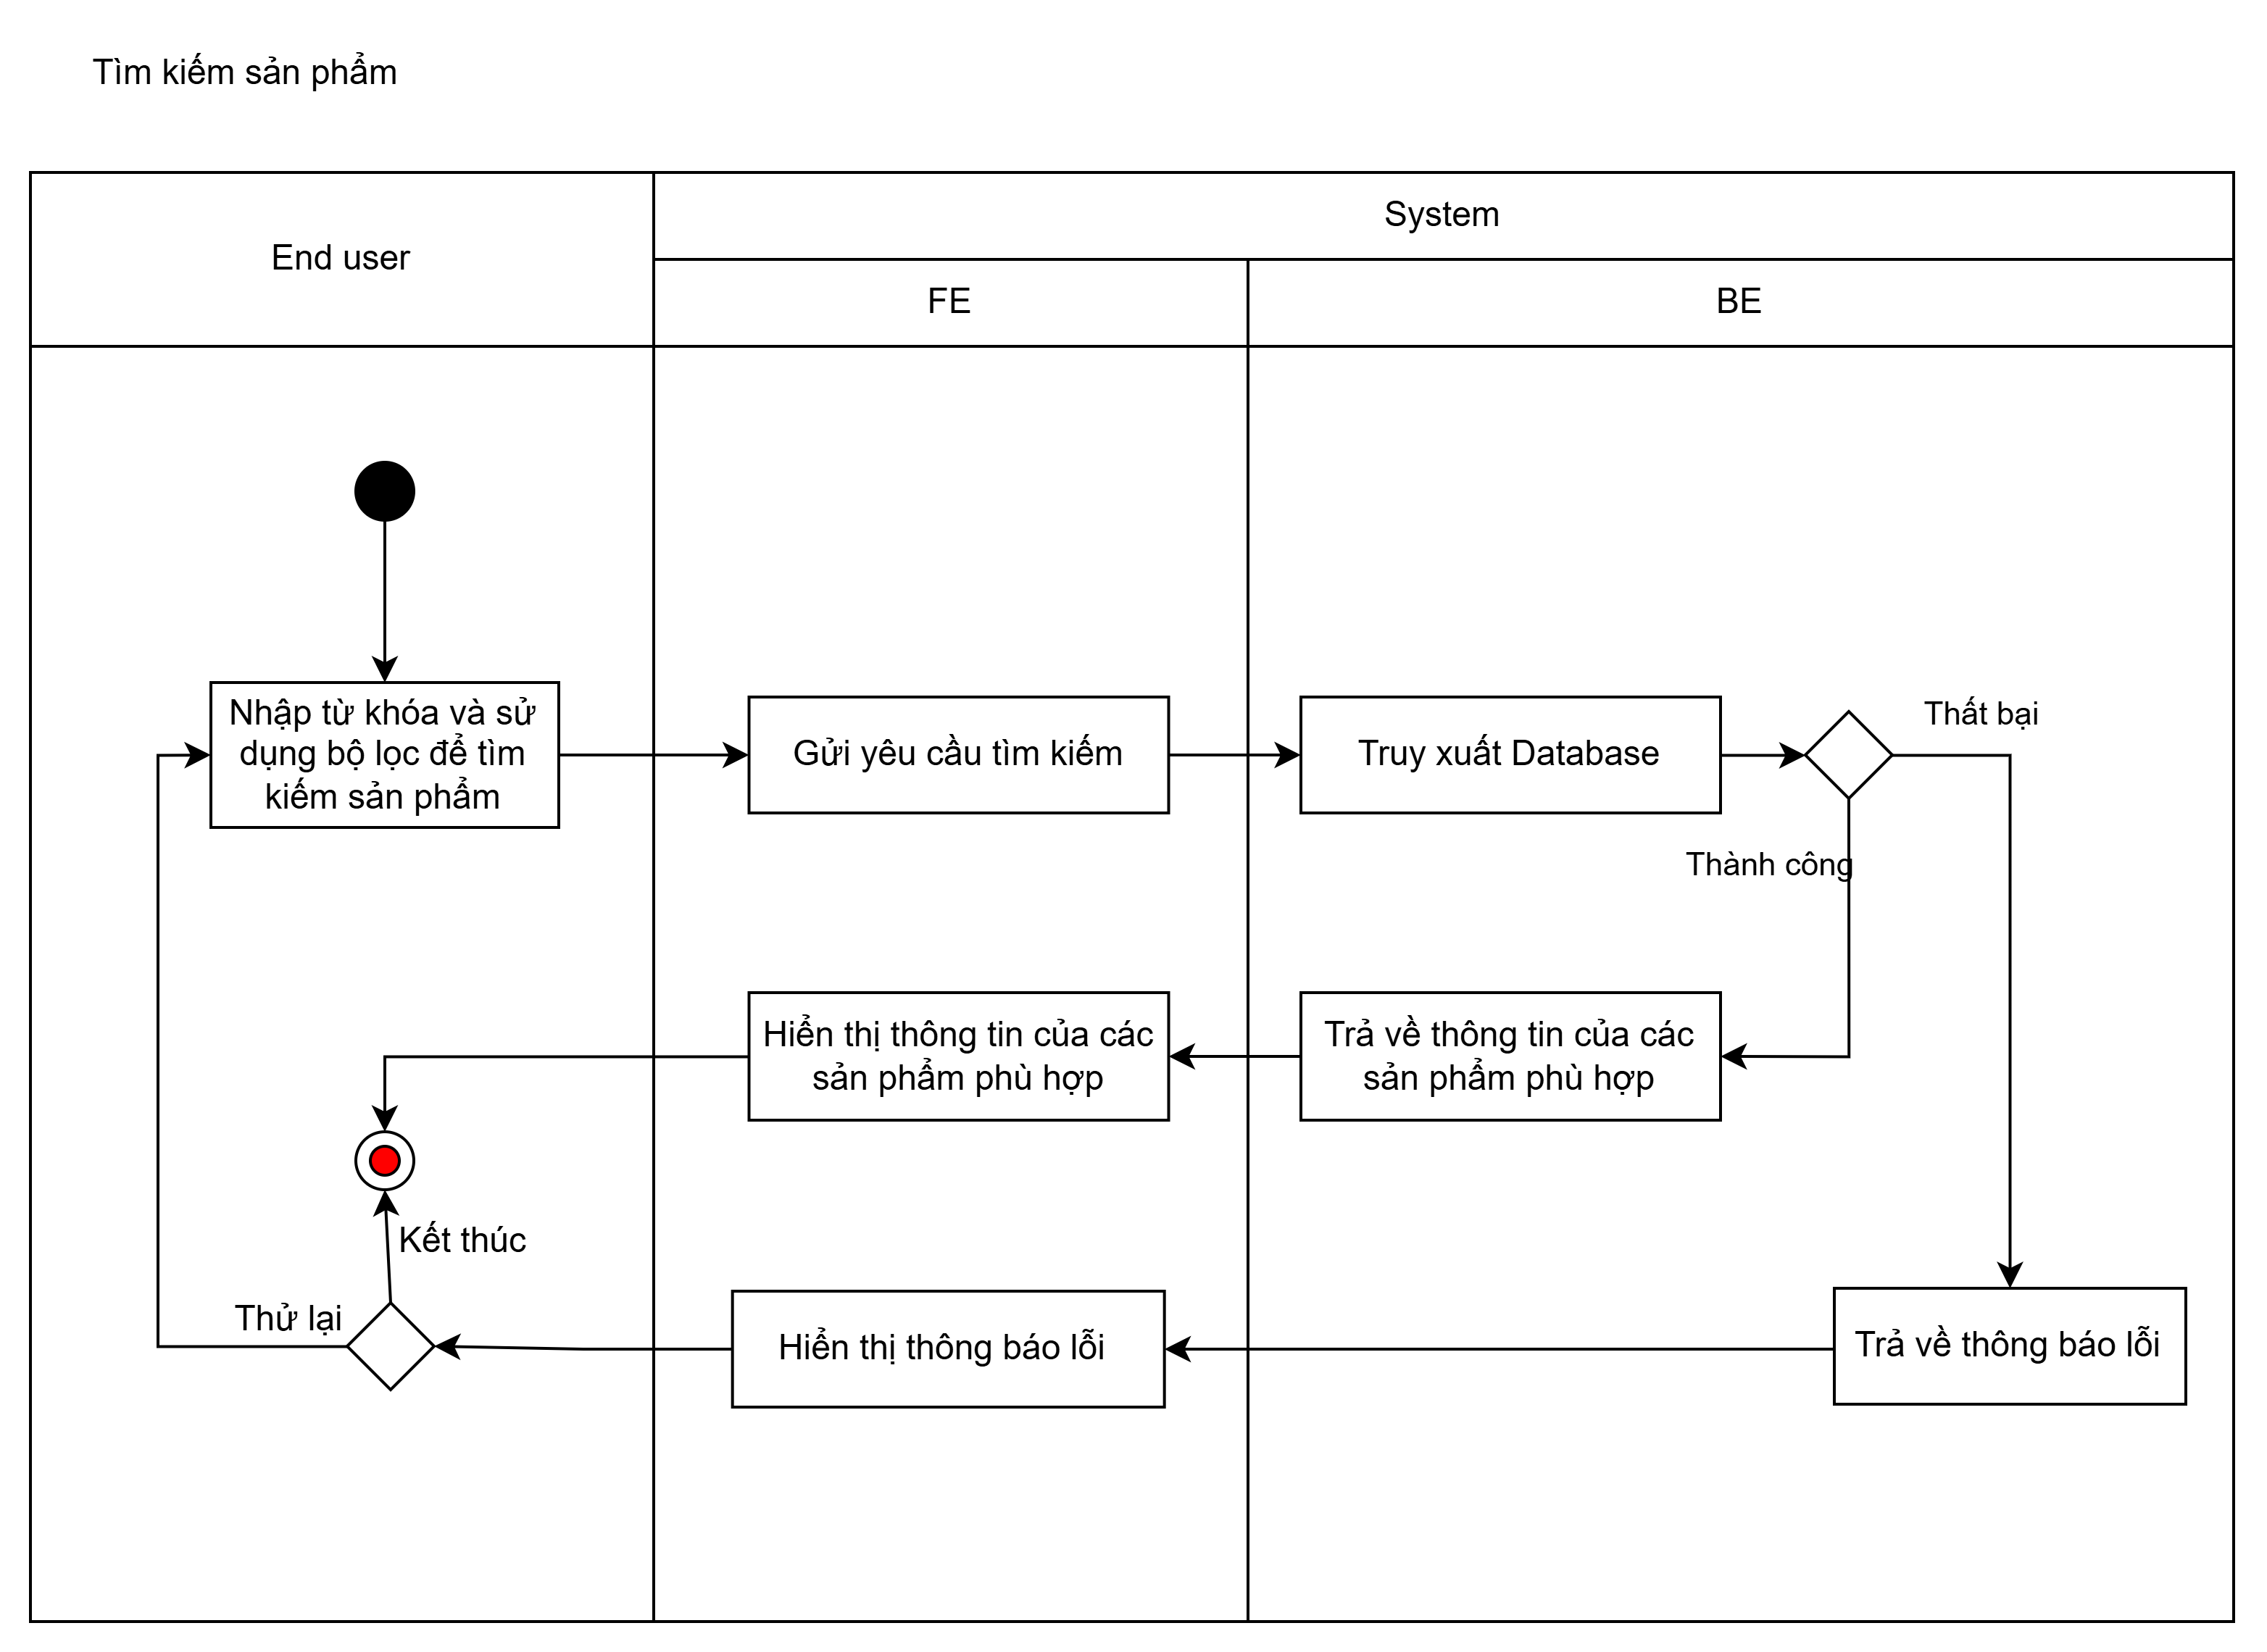
\includegraphics[width=0.8\linewidth]{images/chap3/activity_diagram/find_product.png}
   \vspace{0.5cm} \caption{Sơ đồ hoạt động Tìm kiếm sản phẩm}
    \label{fig:act_find_product}
\end{figure}
Mô tả luồng người dùng nhập từ khóa hoặc chọn danh mục, hệ thống lọc dữ liệu và hiển thị danh sách sản phẩm phù hợp cùng chi tiết sản phẩm.

\begin{figure}[H]
    \centering
    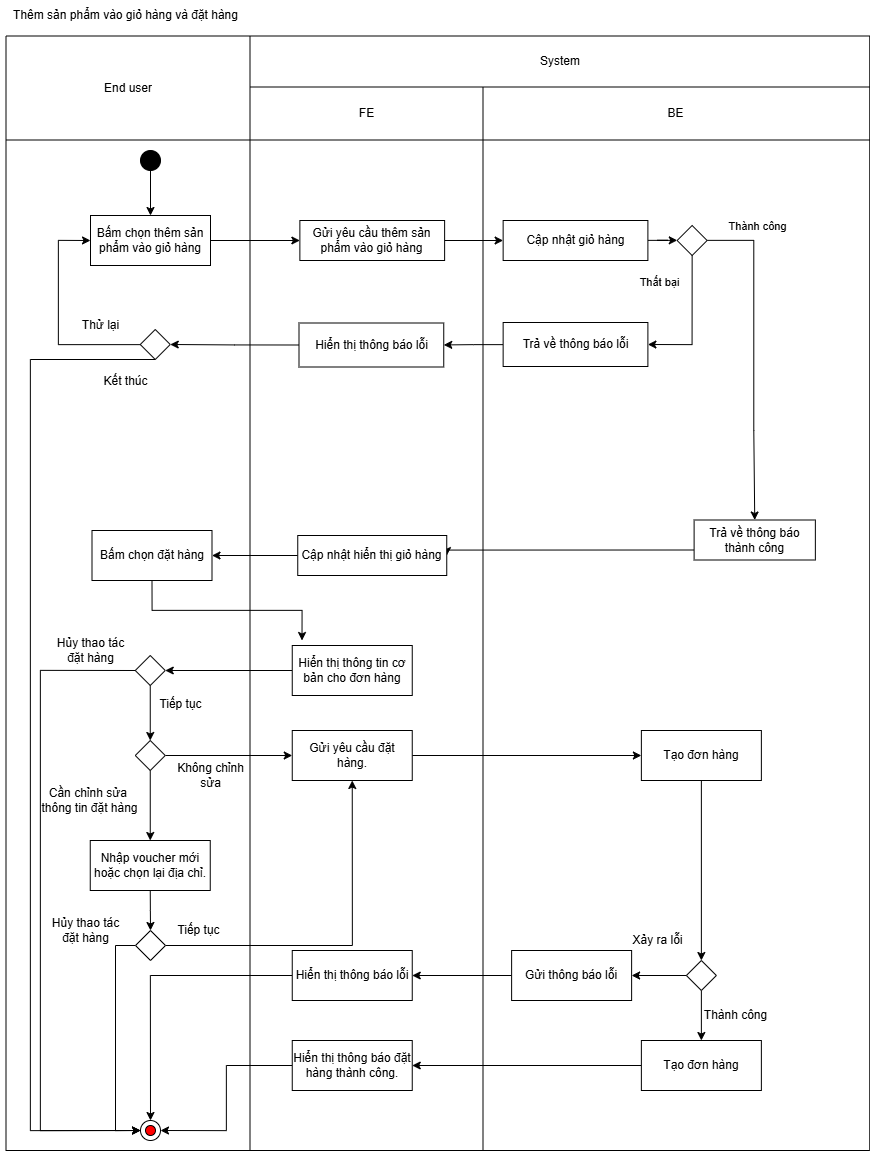
\includegraphics[width=0.8\linewidth]{images/chap3/activity_diagram/add_to_cart_and_checkout.png}
   \vspace{0.5cm} \caption{Sơ đồ hoạt động Thêm vào giỏ hàng và Đặt hàng}
    \label{fig:act_cart_checkout}
\end{figure}
Quy trình cốt lõi: Người dùng chọn sản phẩm, thêm vào giỏ, kiểm tra lại giỏ hàng, nhập thông tin giao hàng và xác nhận tạo đơn hàng.

\begin{figure}[H]
    \centering
    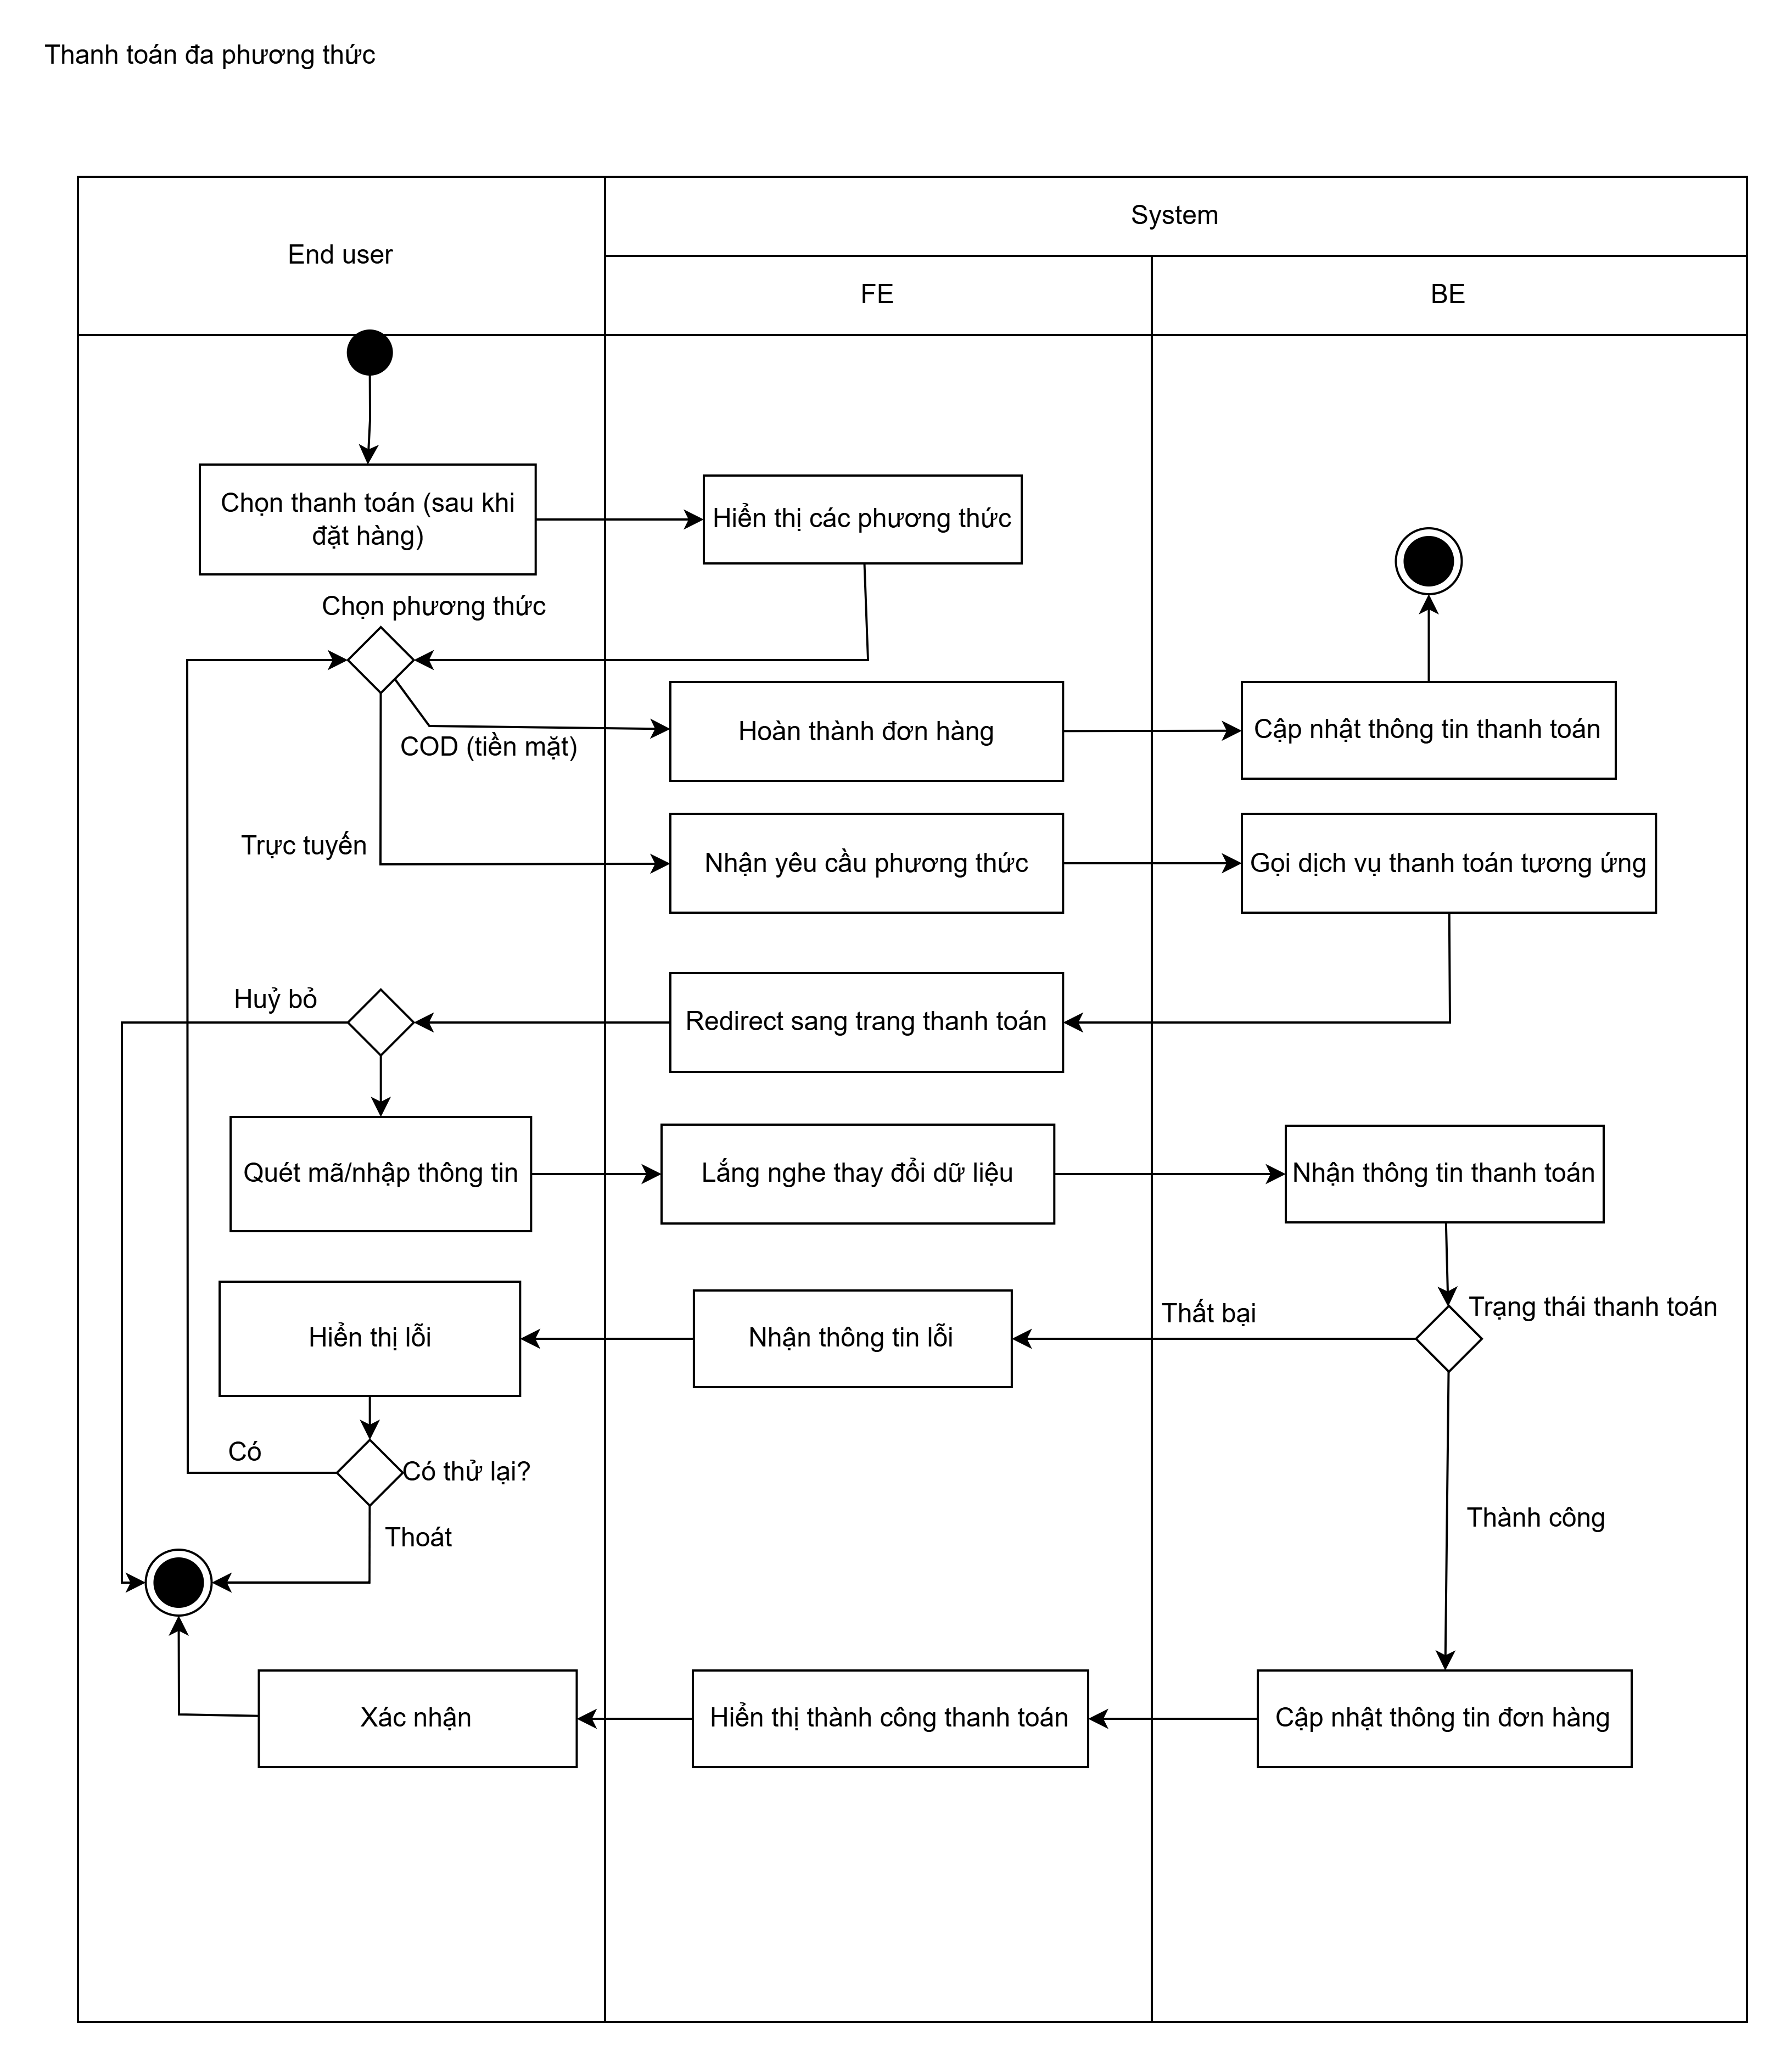
\includegraphics[width=0.8\linewidth]{images/chap3/activity_diagram/multiple_payment_method.png}
   \vspace{0.5cm} \caption{Sơ đồ hoạt động Lựa chọn phương thức thanh toán}
    \label{fig:act_payment}
\end{figure}
Chi tiết hóa bước thanh toán, cho phép người dùng chọn giữa các phương thức (COD, Ví điện tử, Chuyển khoản) và xử lý luồng giao dịch tương ứng.

% --- PHẦN 3: QUẢN LÝ ĐƠN HÀNG (ORDER MANAGEMENT) ---

\begin{figure}[H]
    \centering
    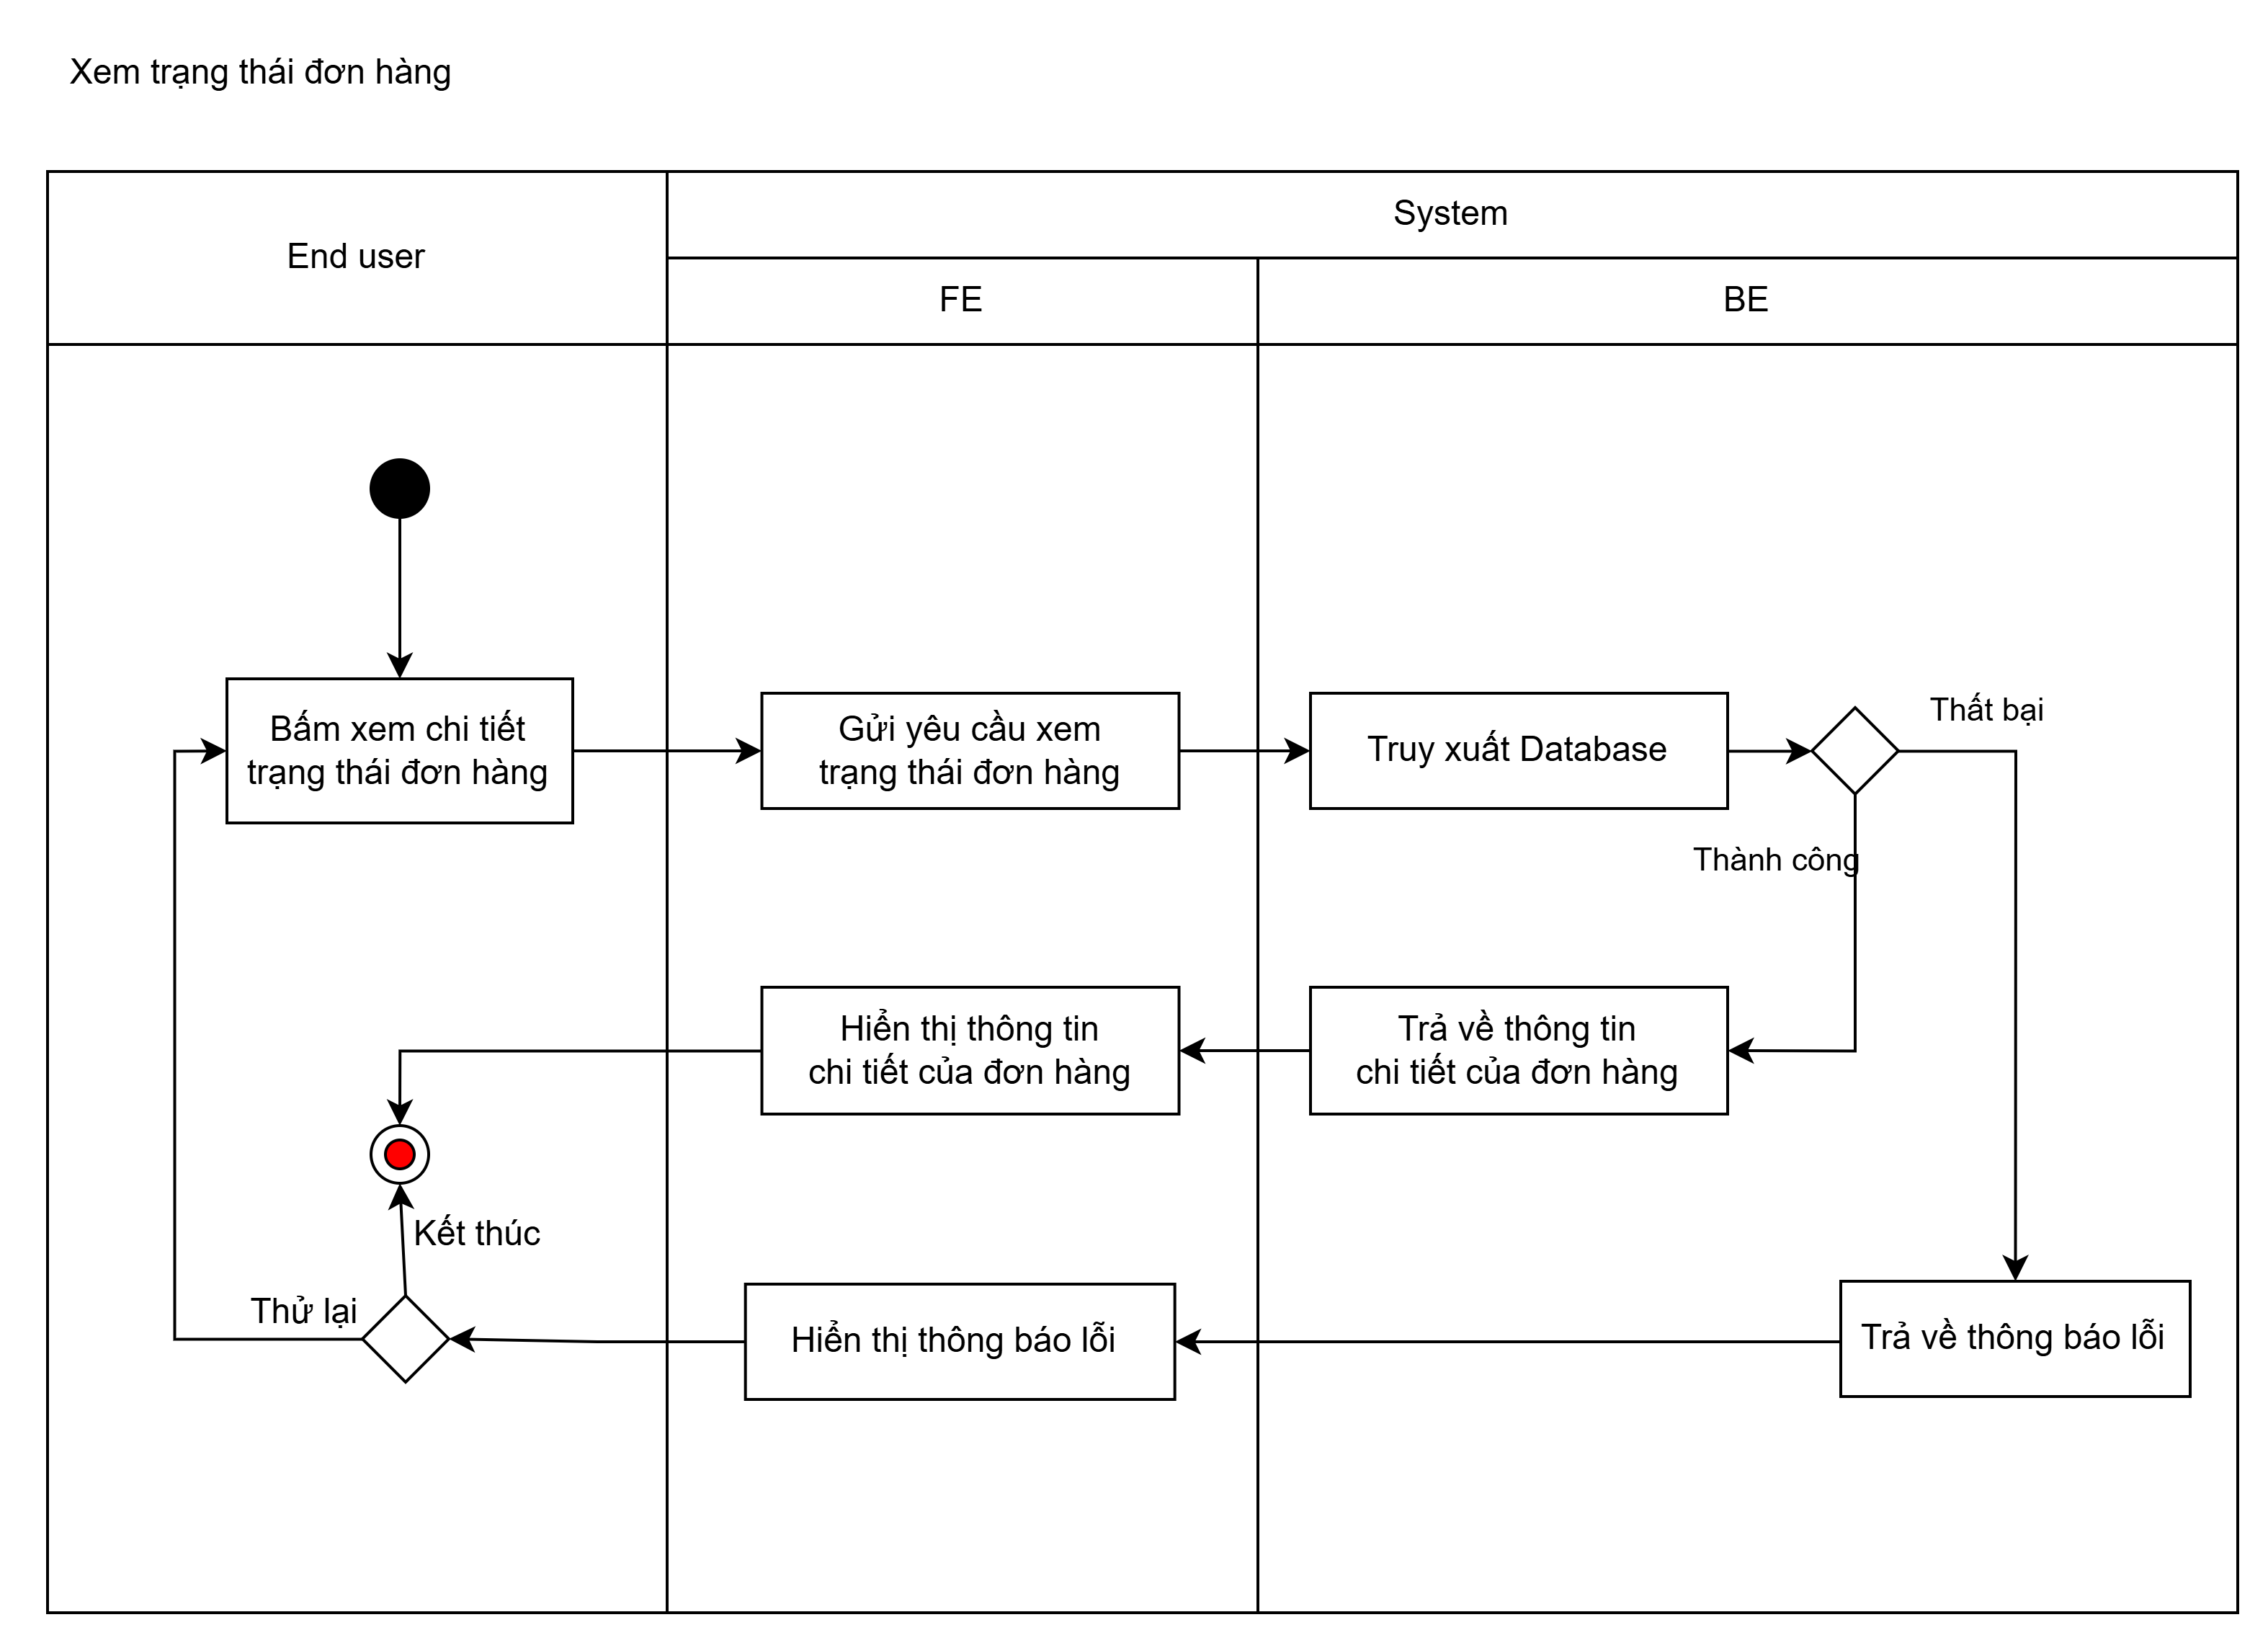
\includegraphics[width=0.8\linewidth]{images/chap3/activity_diagram/view_order_status.png}
   \vspace{0.5cm} \caption{Sơ đồ hoạt động Xem trạng thái đơn hàng}
    \label{fig:act_view_order}
\end{figure}
Người dùng theo dõi tiến trình của đơn hàng đã đặt (Chờ xác nhận, Đang giao, Đã giao, v.v.) thông qua giao diện lịch sử mua hàng.

\begin{figure}[H]
    \centering
    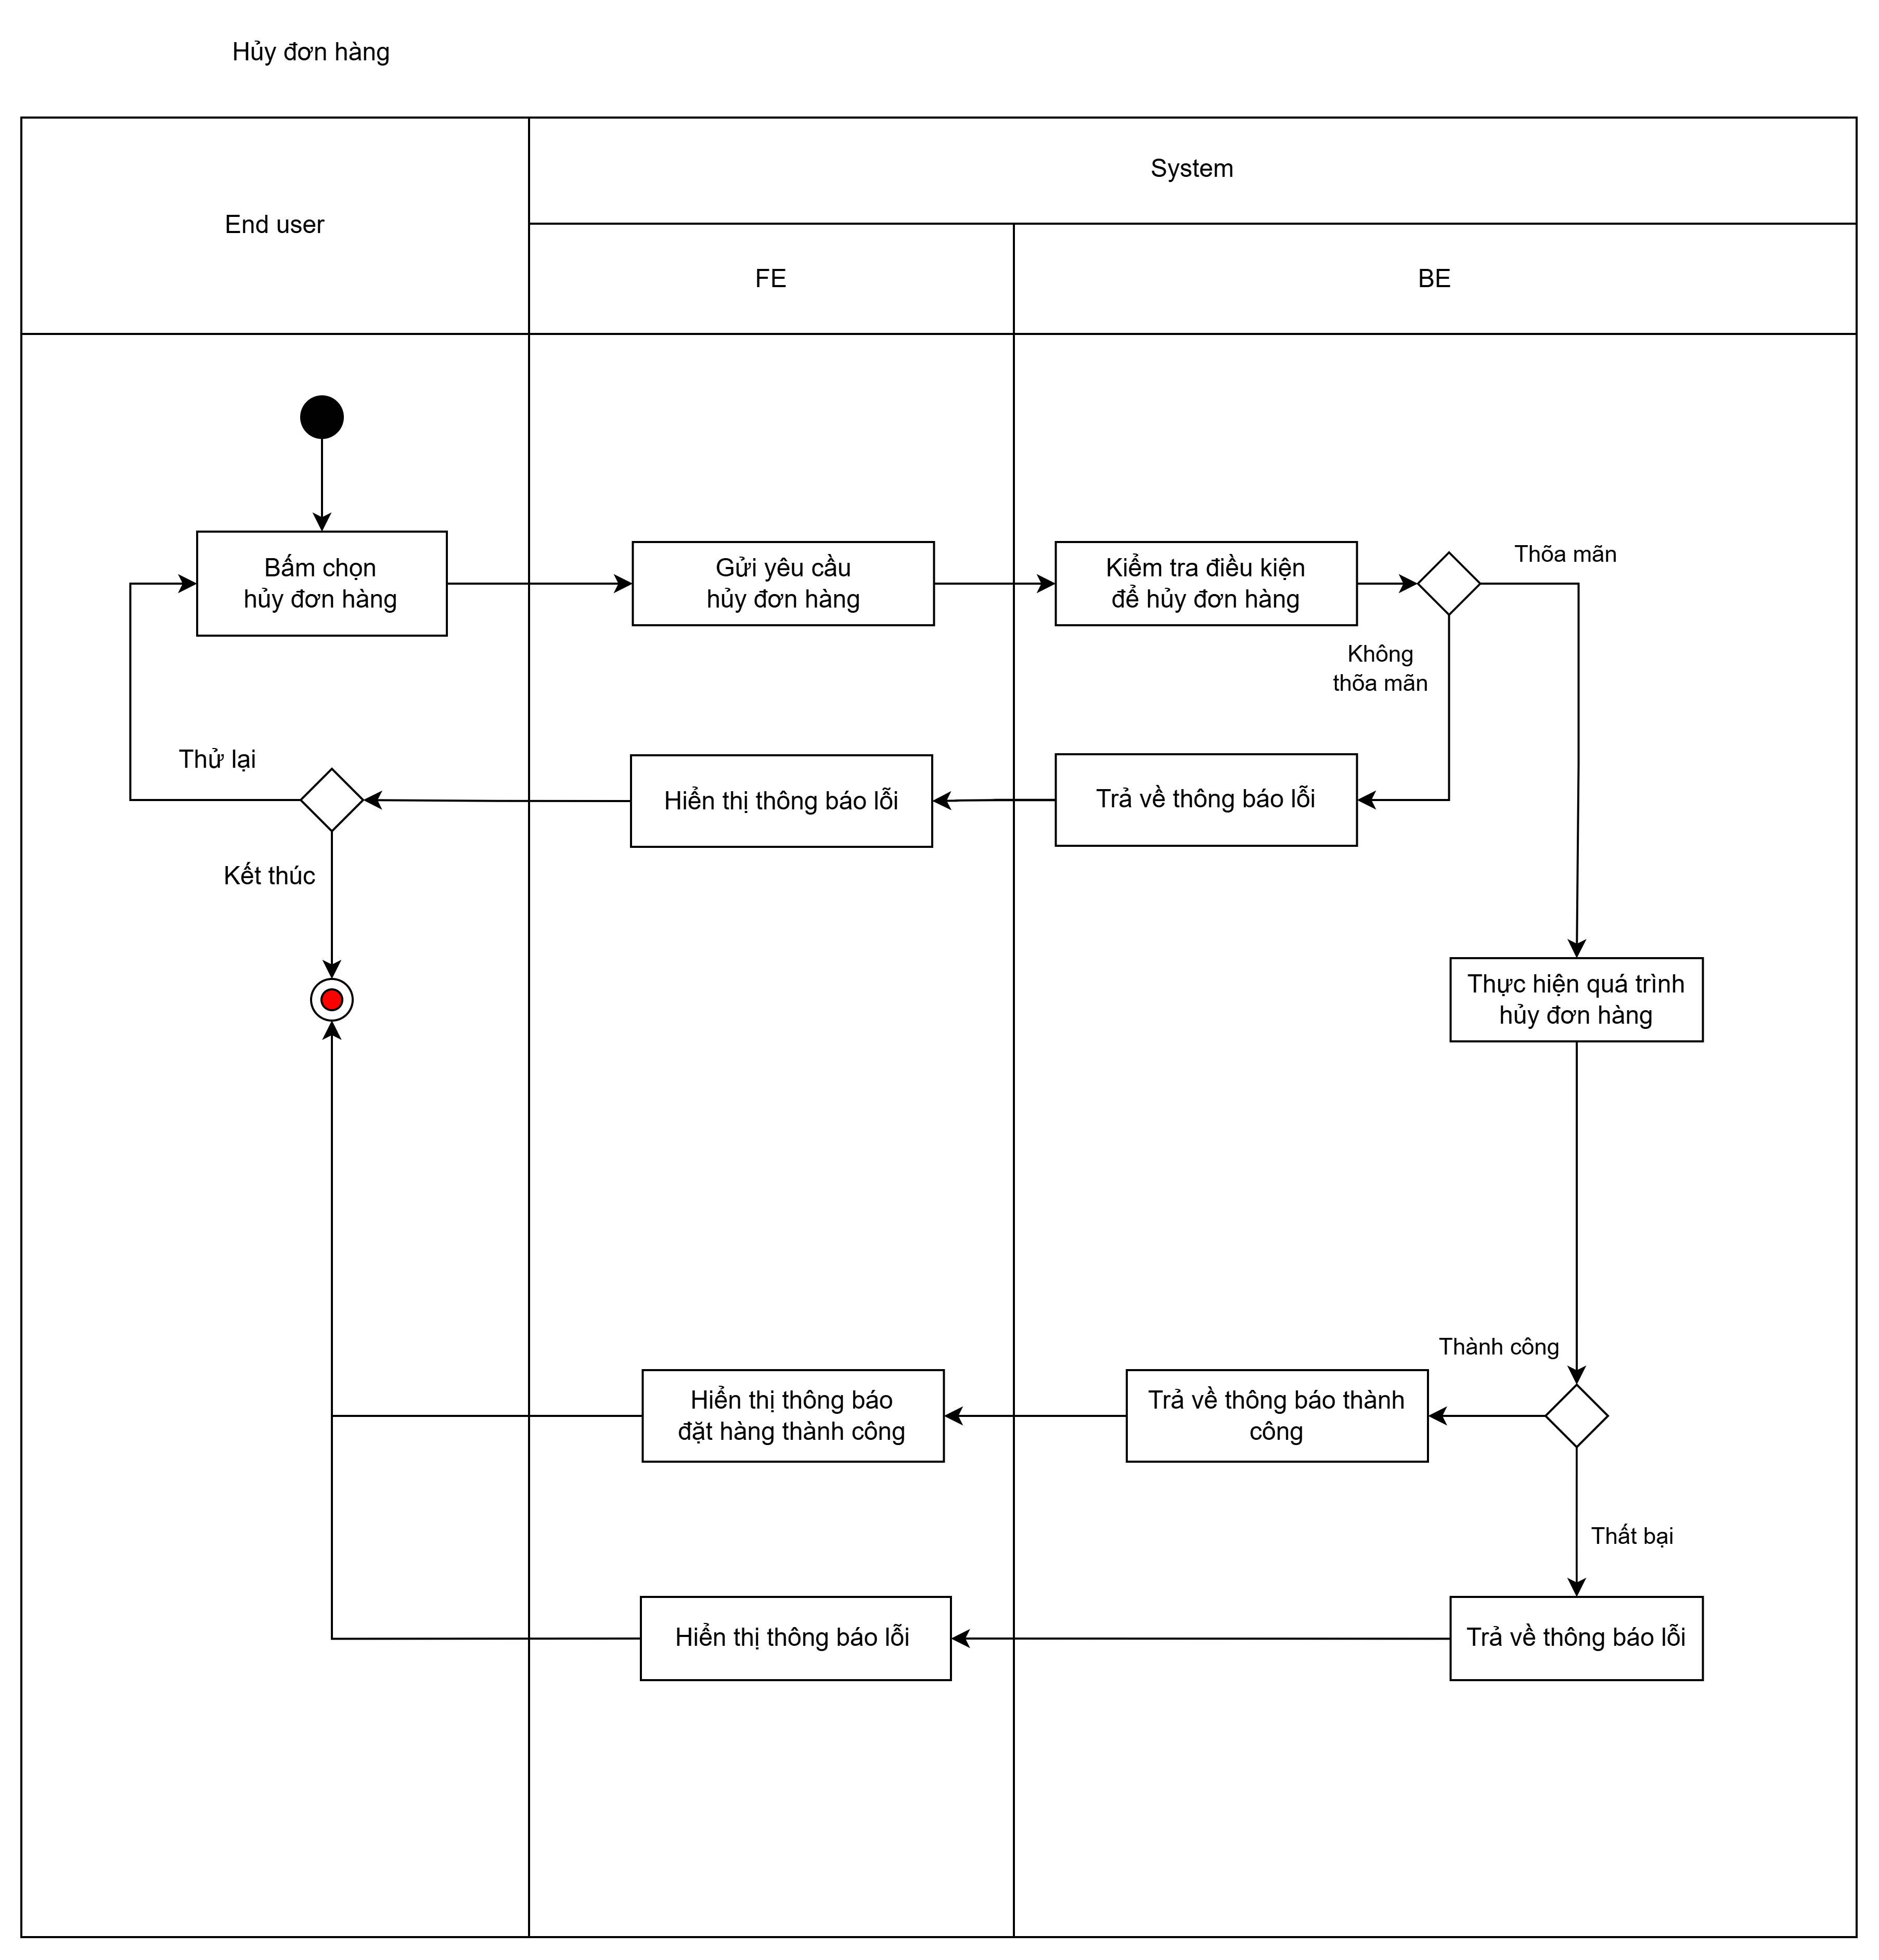
\includegraphics[width=0.7\linewidth]{images/chap3/activity_diagram/cancel_order.png}
   \vspace{0.5cm} \caption{Sơ đồ hoạt động Hủy đơn hàng (Phía người dùng)}
    \label{fig:act_cancel_order}
\end{figure}
Quy trình cho phép người dùng yêu cầu hủy đơn hàng khi đơn chưa được chuyển sang trạng thái vận chuyển, hệ thống cập nhật trạng thái và hoàn tiền (nếu có).

% --- PHẦN 4: HỖ TRỢ KHÁCH HÀNG (CUSTOMER SUPPORT) ---

\begin{figure}[H]
    \centering
    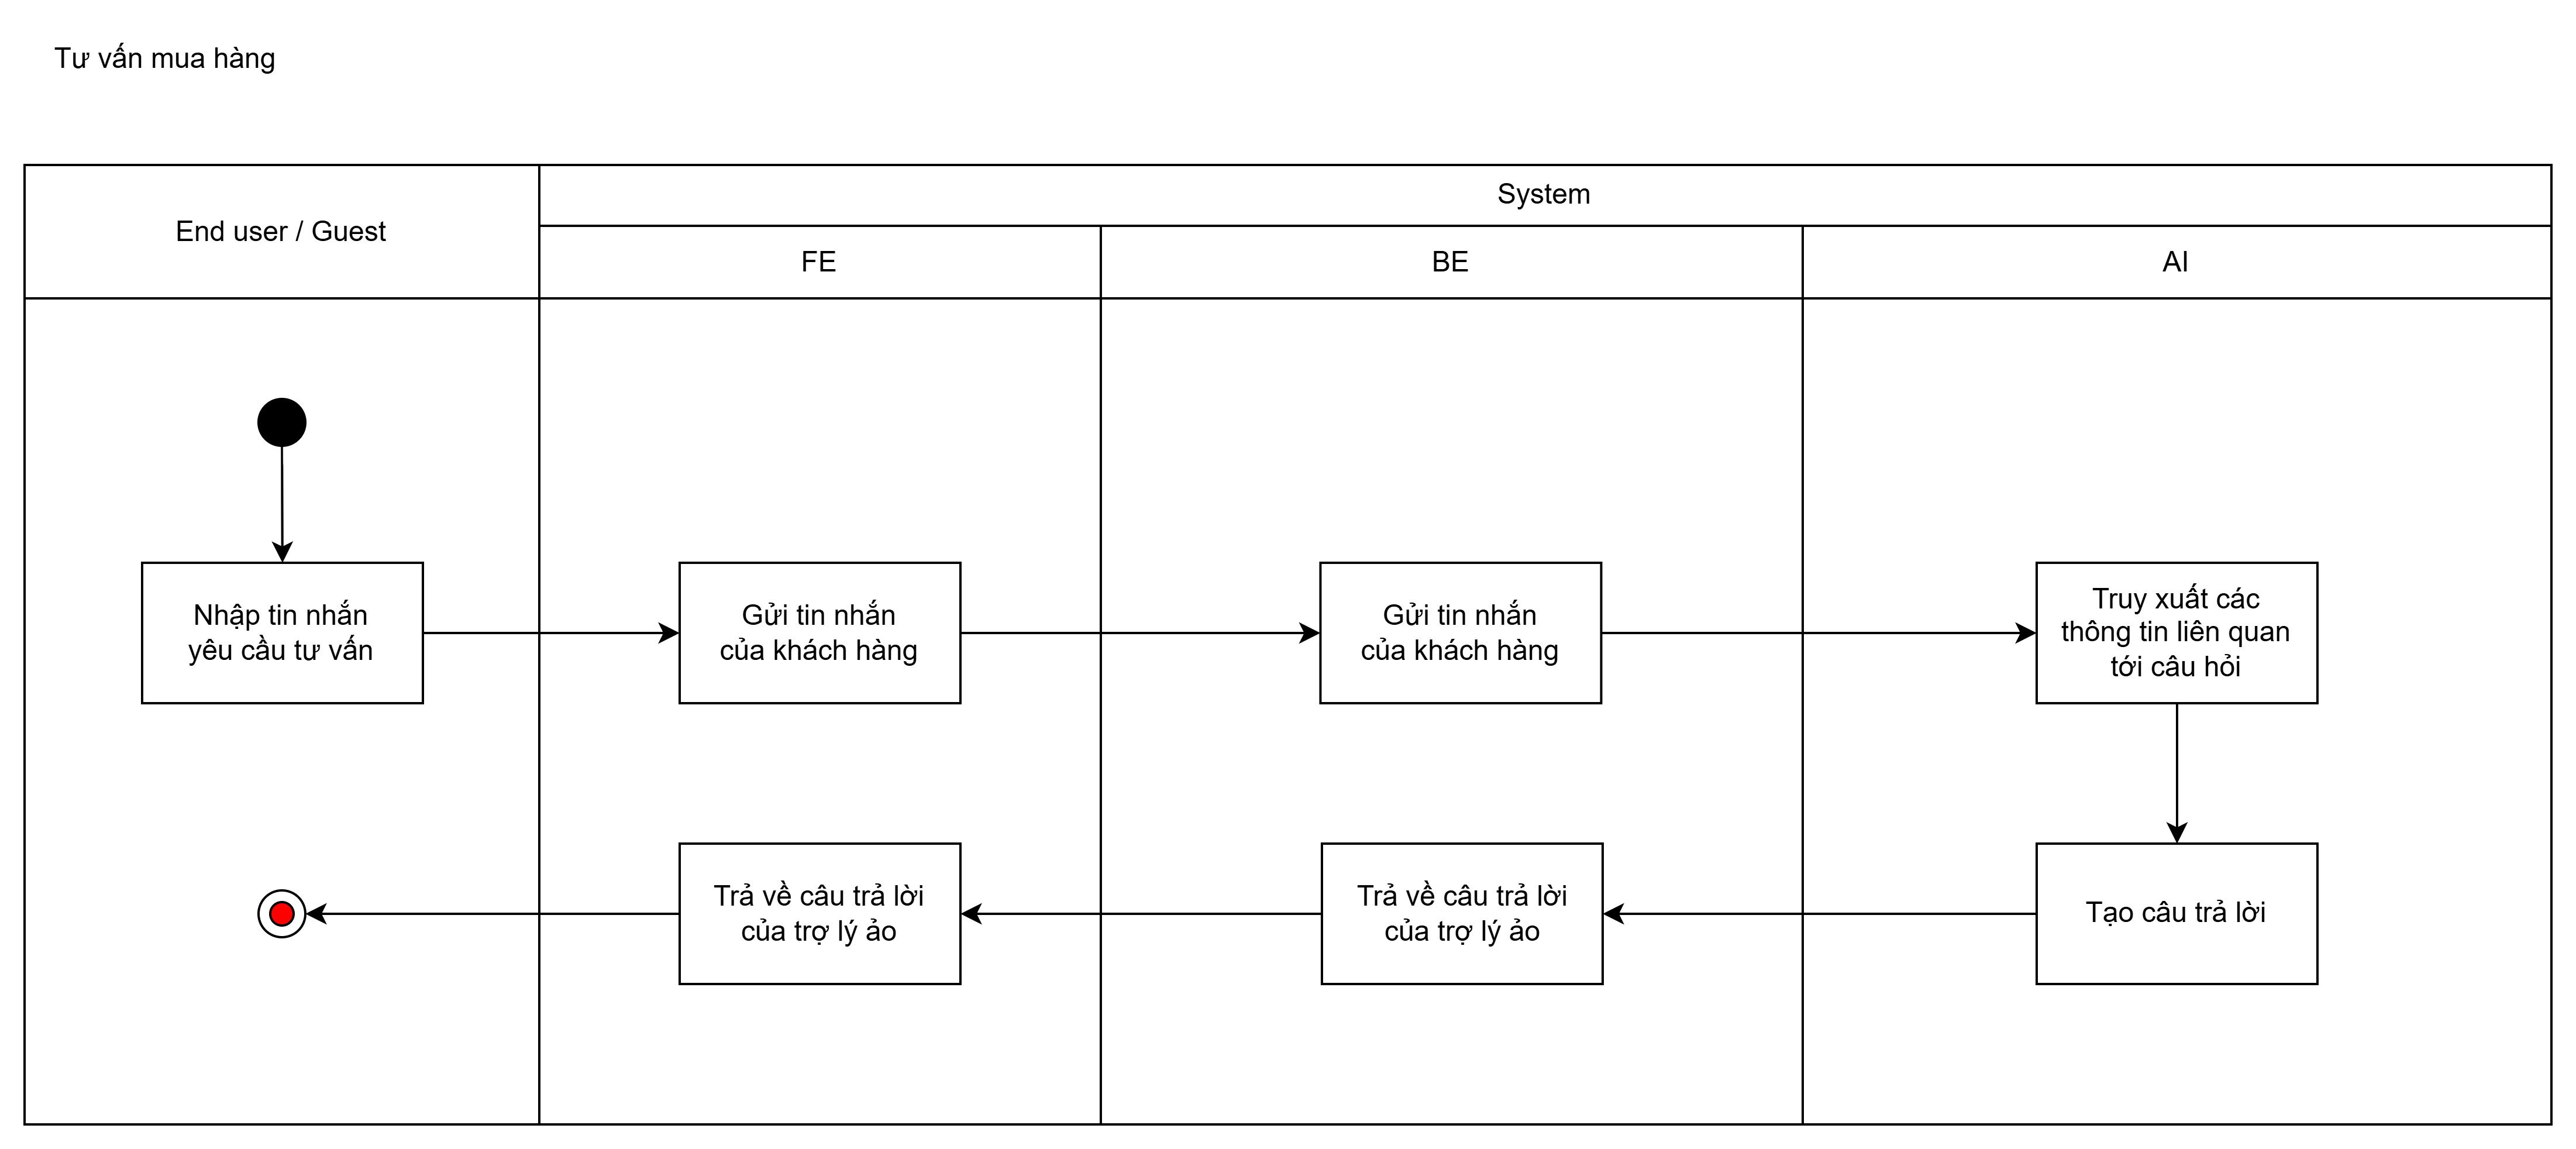
\includegraphics[width=0.8\linewidth]{images/chap3/activity_diagram/shopping_consulting.png}
   \vspace{0.5cm} \caption{Sơ đồ hoạt động Tư vấn mua sắm}
    \label{fig:act_consulting}
\end{figure}
Mô tả tương tác giữa khách hàng và nhân viên/chatbot để nhận tư vấn về thông tin sản phẩm trước khi quyết định mua.

\begin{figure}[H]
    \centering
    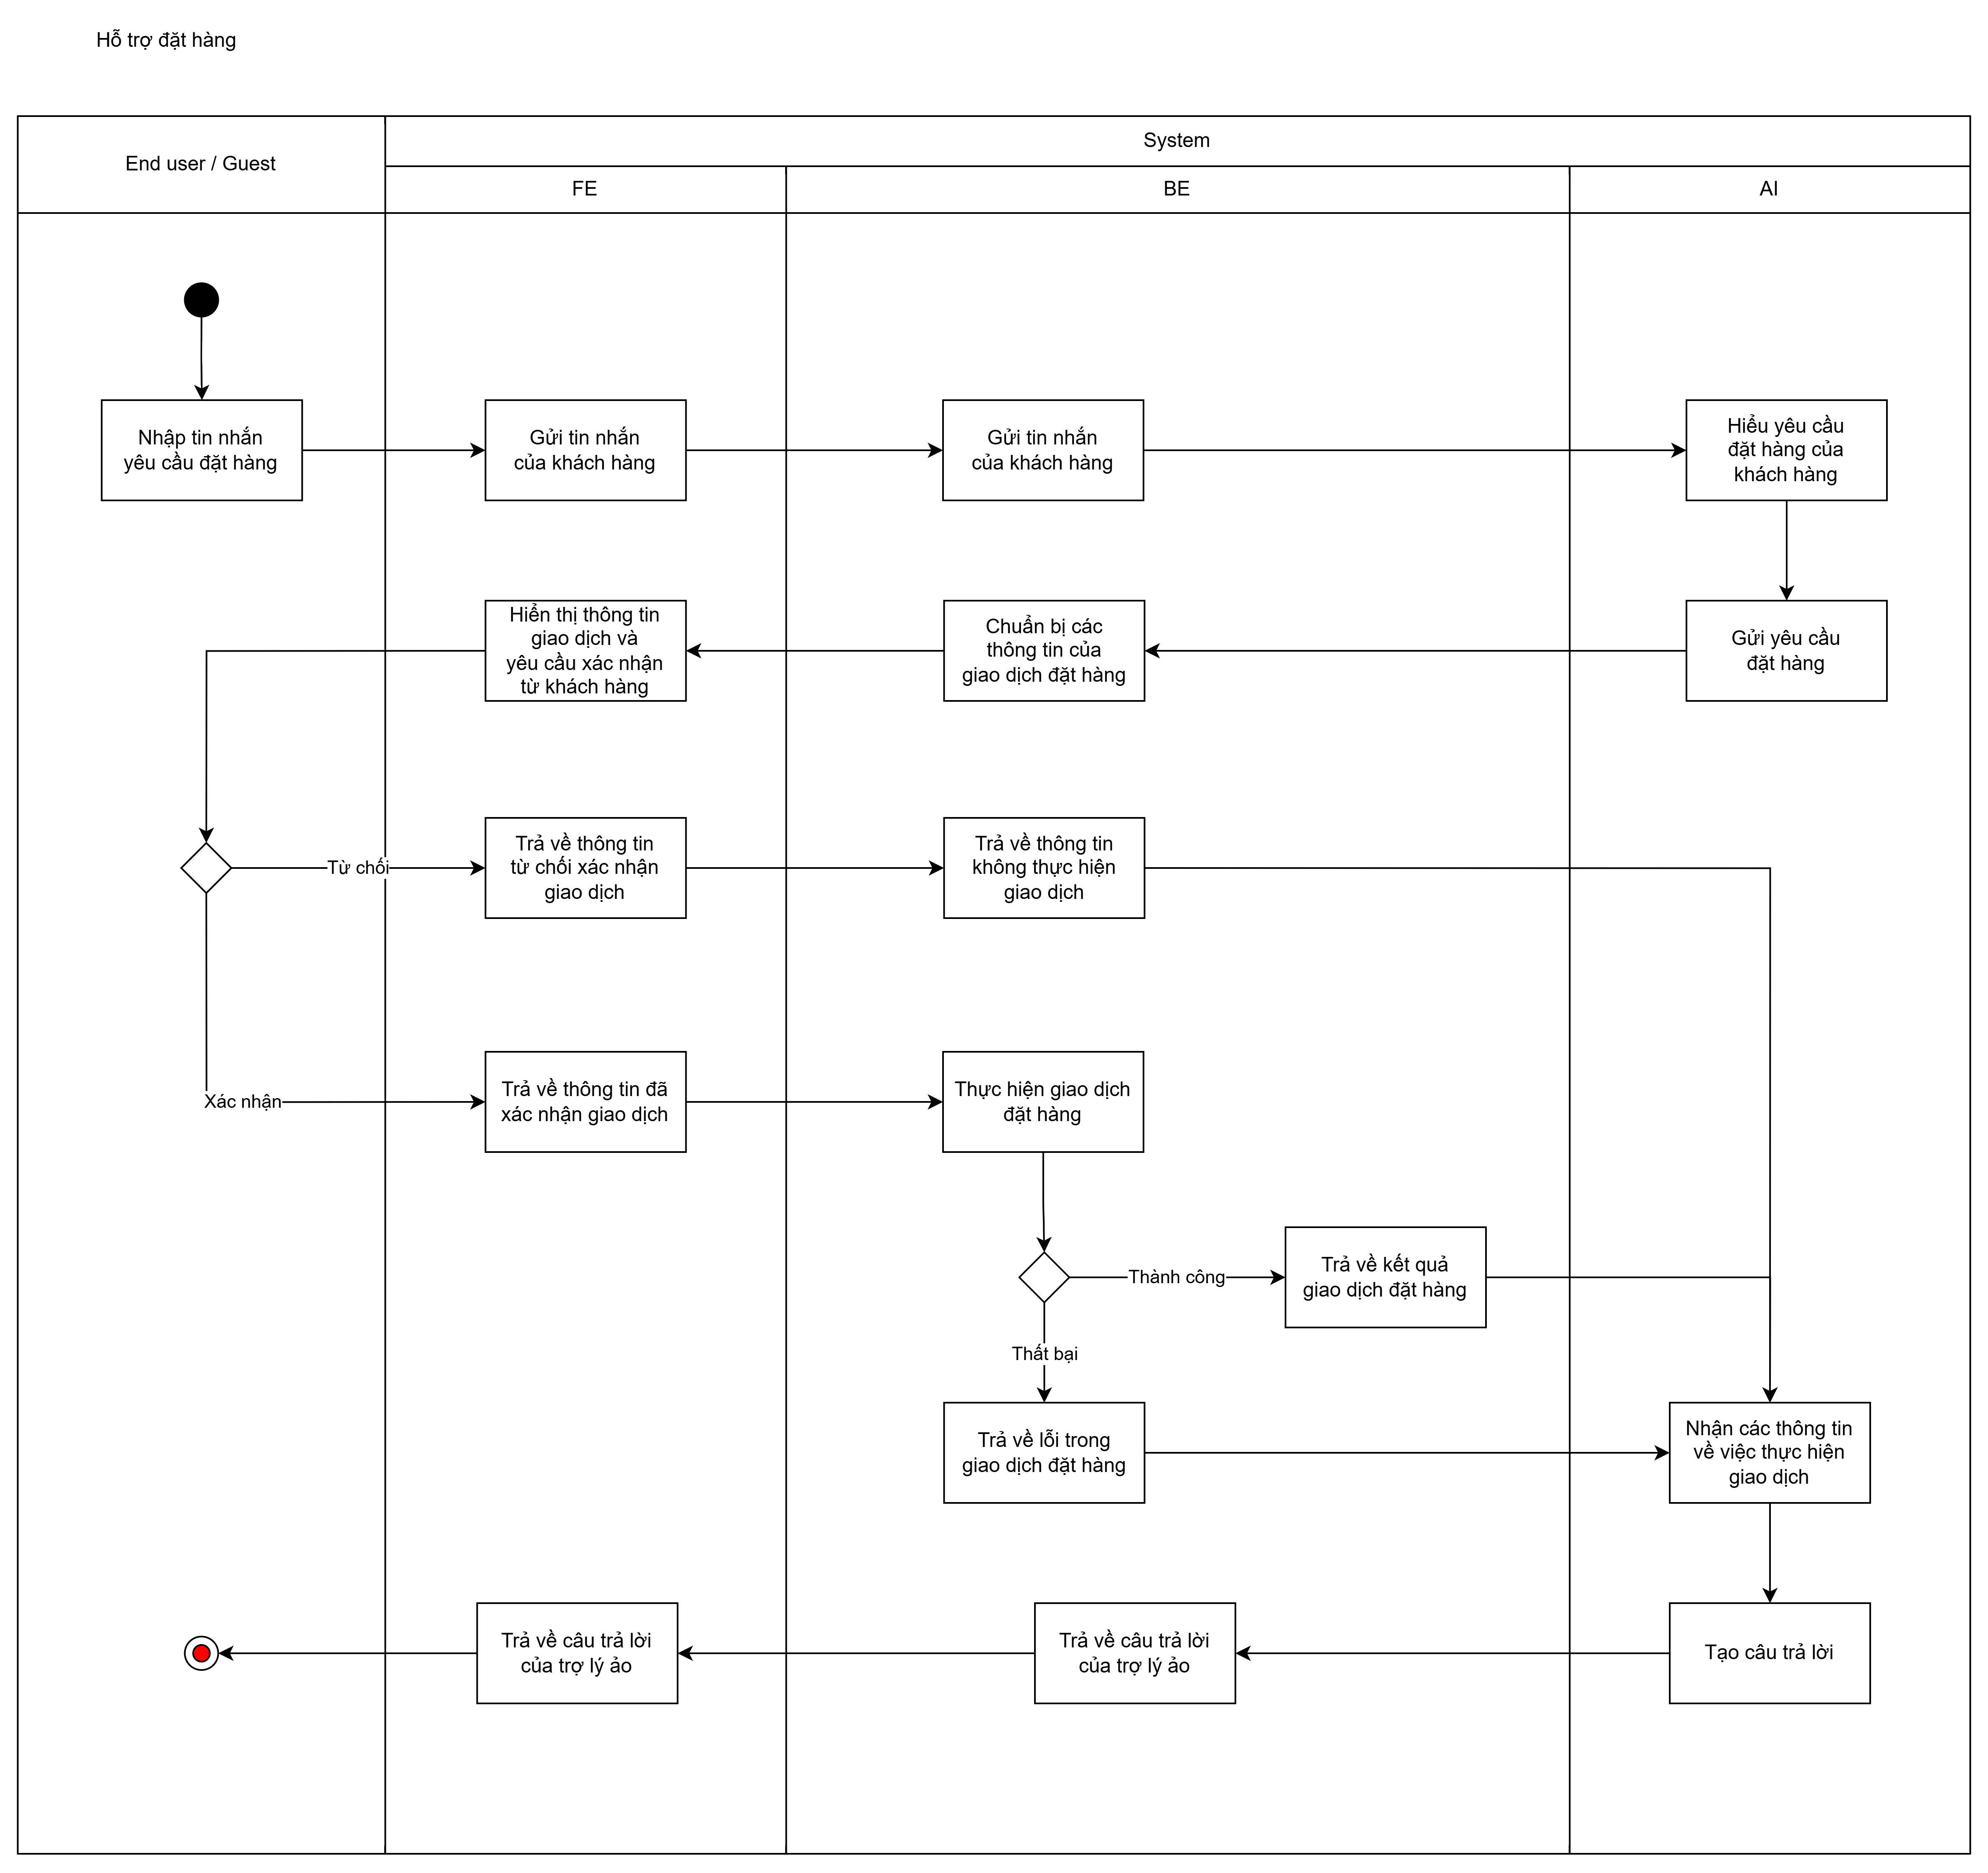
\includegraphics[width=0.8\linewidth]{images/chap3/activity_diagram/place_order_support.png}
   \vspace{0.5cm} \caption{Sơ đồ hoạt động Hỗ trợ đặt hàng}
    \label{fig:act_support_place_order}
\end{figure}
Quy trình hỗ trợ khi người dùng gặp khó khăn trong thao tác đặt hàng, nhân viên hỗ trợ có thể hướng dẫn hoặc tạo đơn hộ.

\begin{figure}[H]
    \centering
    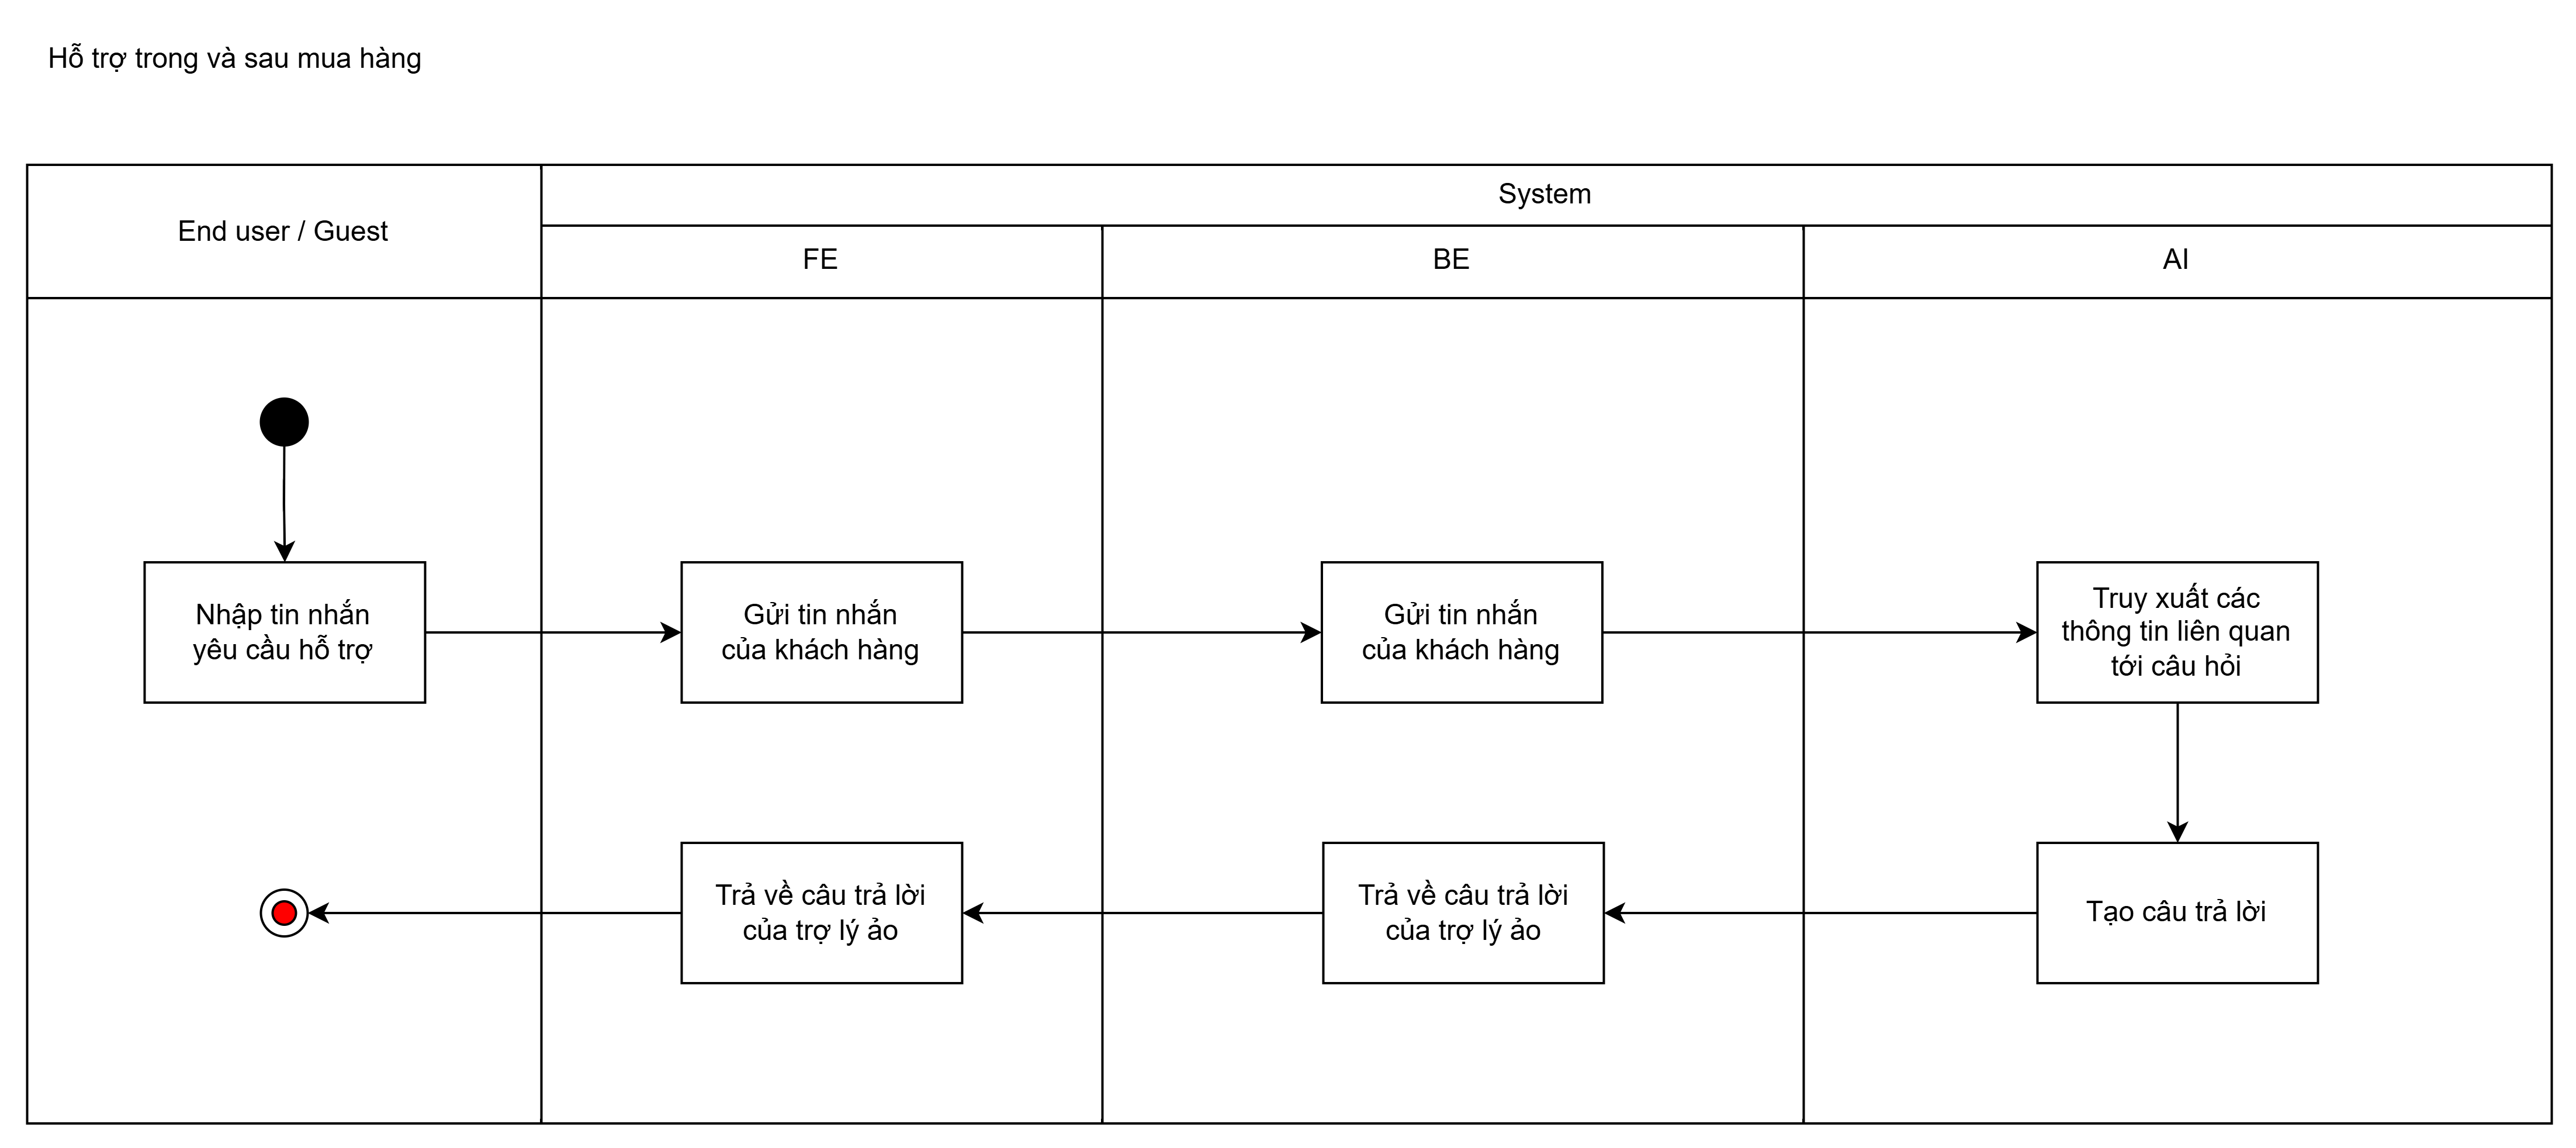
\includegraphics[width=0.8\linewidth]{images/chap3/activity_diagram/shopping_support.png}
   \vspace{0.5cm} \caption{Sơ đồ hoạt động Hỗ trợ sau bán hàng}
    \label{fig:act_shopping_support}
\end{figure}
Xử lý các yêu cầu khiếu nại, bảo hành hoặc các vấn đề phát sinh sau khi khách hàng đã nhận được sản phẩm.

\begin{figure}[H]
    \centering
    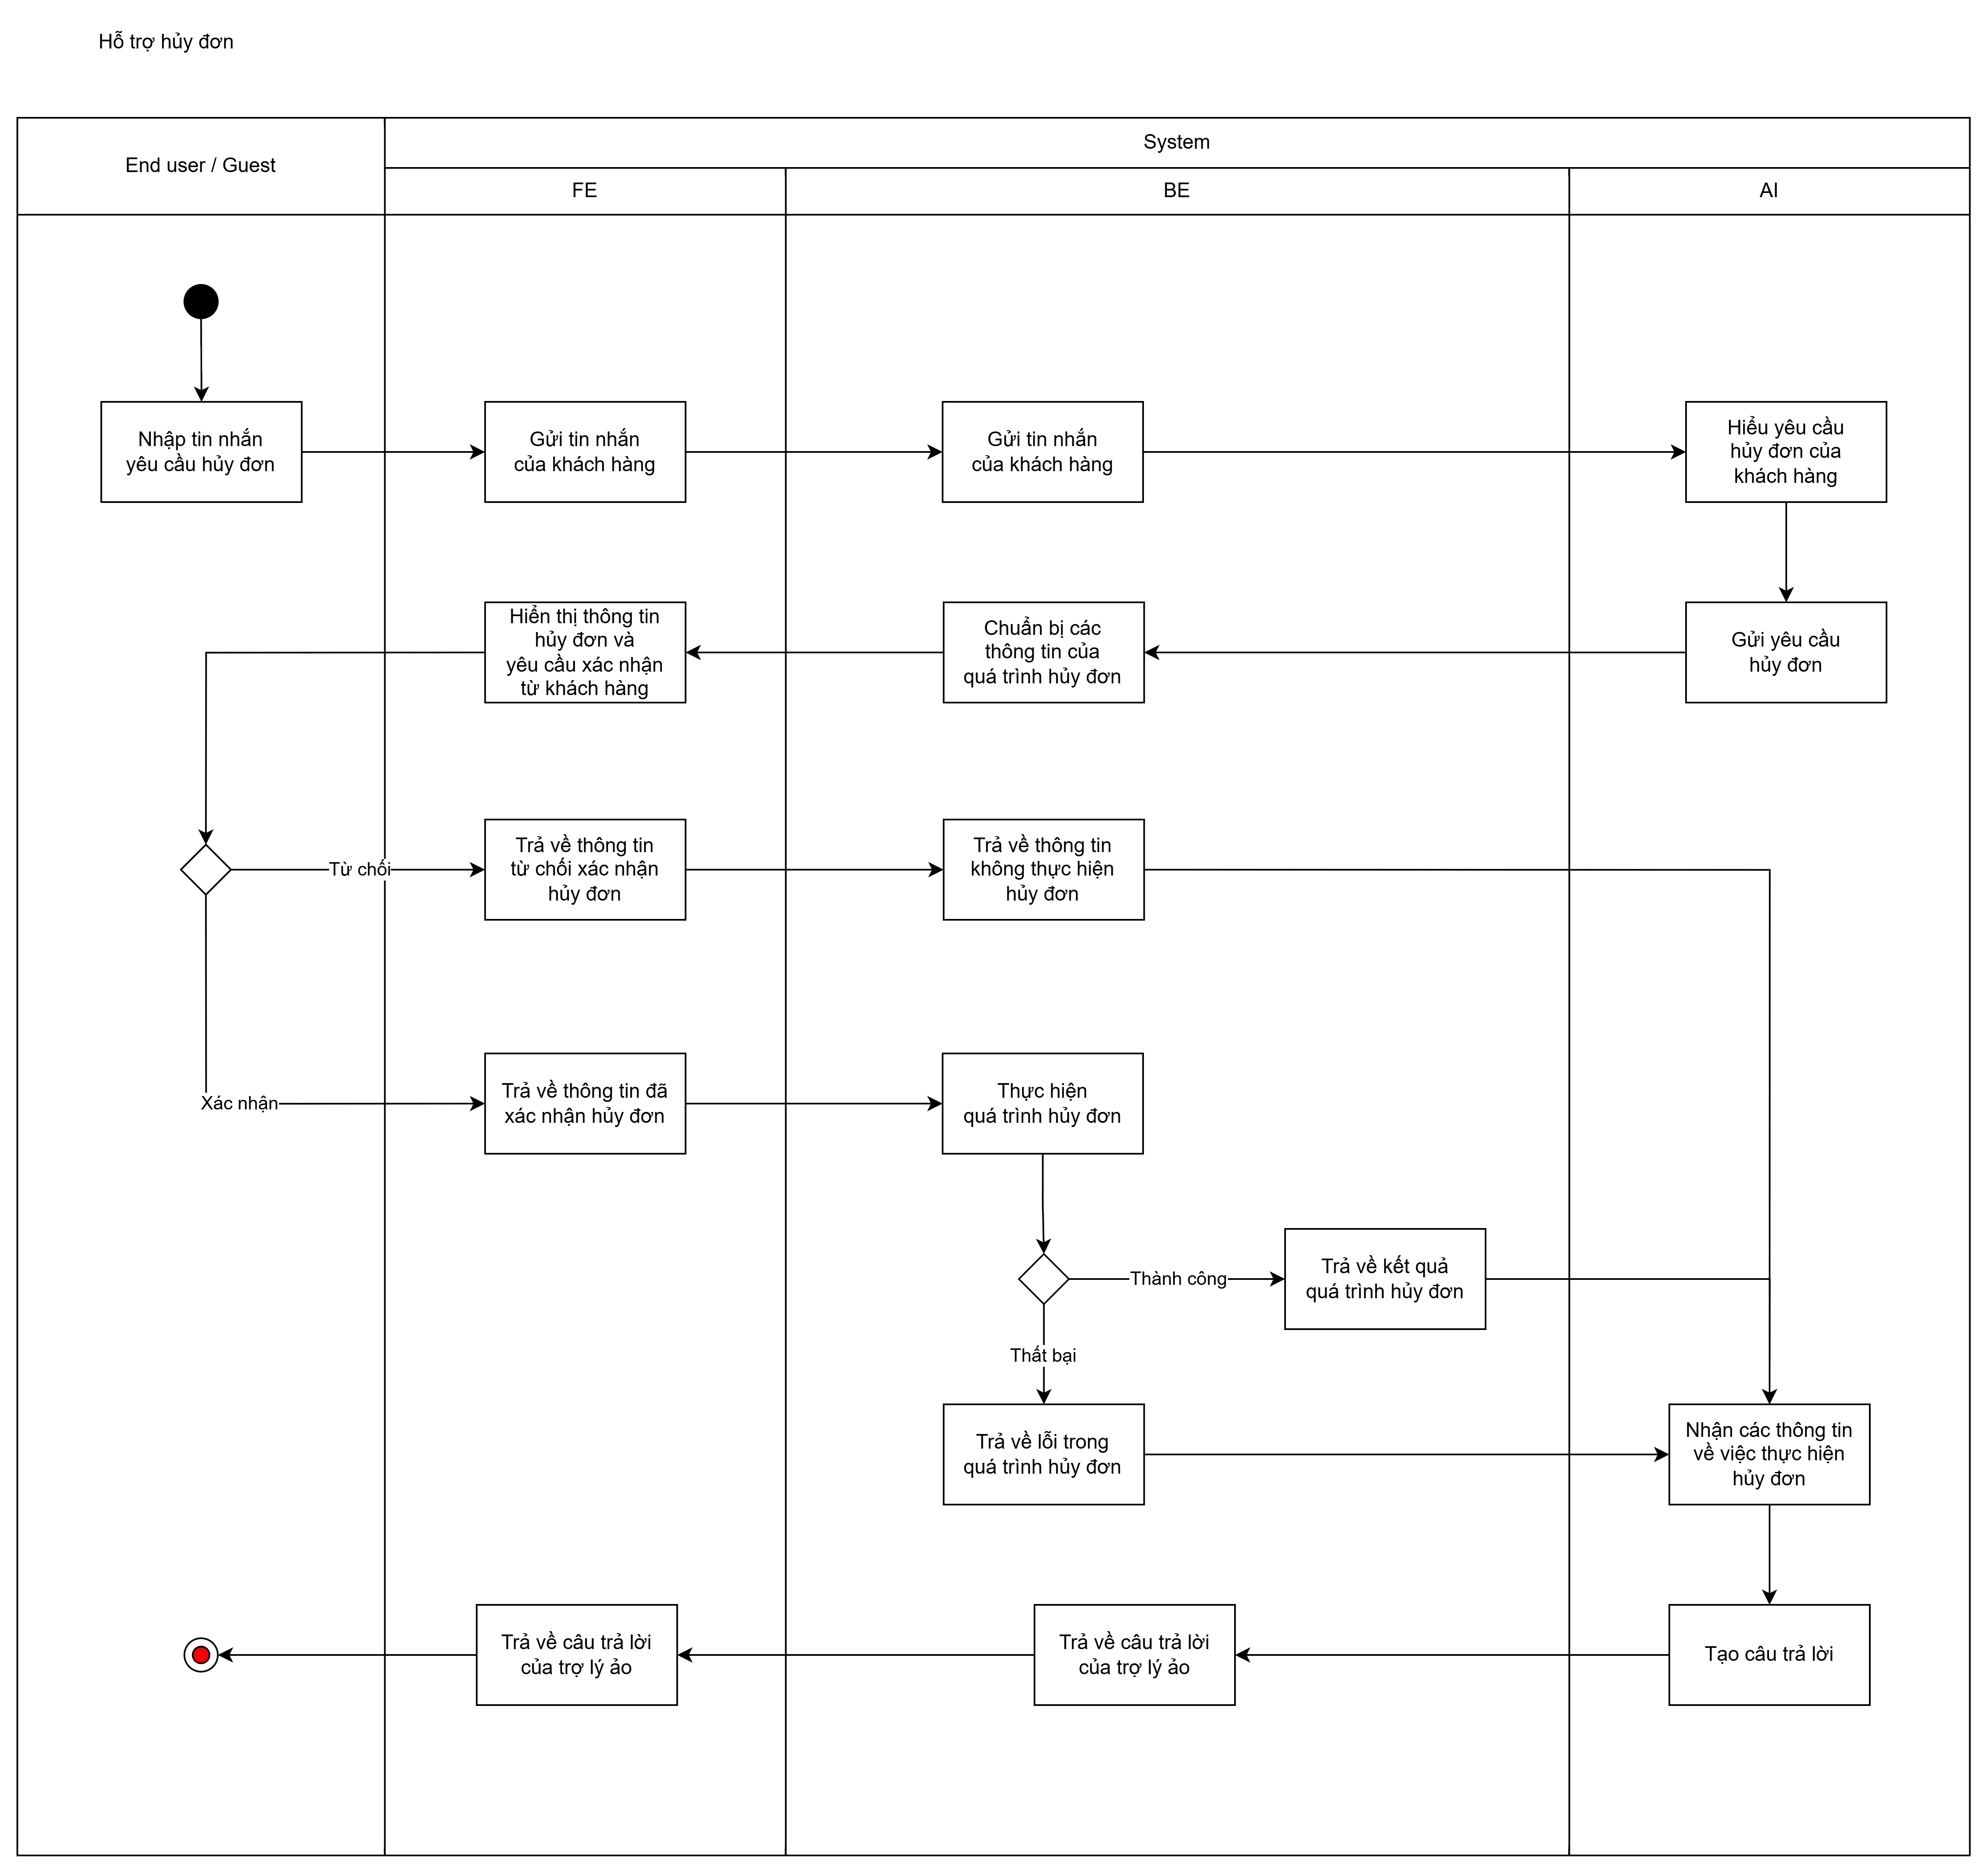
\includegraphics[width=0.8\linewidth]{images/chap3/activity_diagram/cancel_order_support.png}
   \vspace{0.5cm} \caption{Sơ đồ hoạt động Hỗ trợ hủy đơn hàng}
    \label{fig:act_support_cancel}
\end{figure}
Quy trình xử lý phía bộ phận hỗ trợ khi tiếp nhận yêu cầu hủy đơn từ khách hàng (trong trường hợp hệ thống tự động không xử lý được hoặc cần xác minh).

\begin{figure}[H]
    \centering
    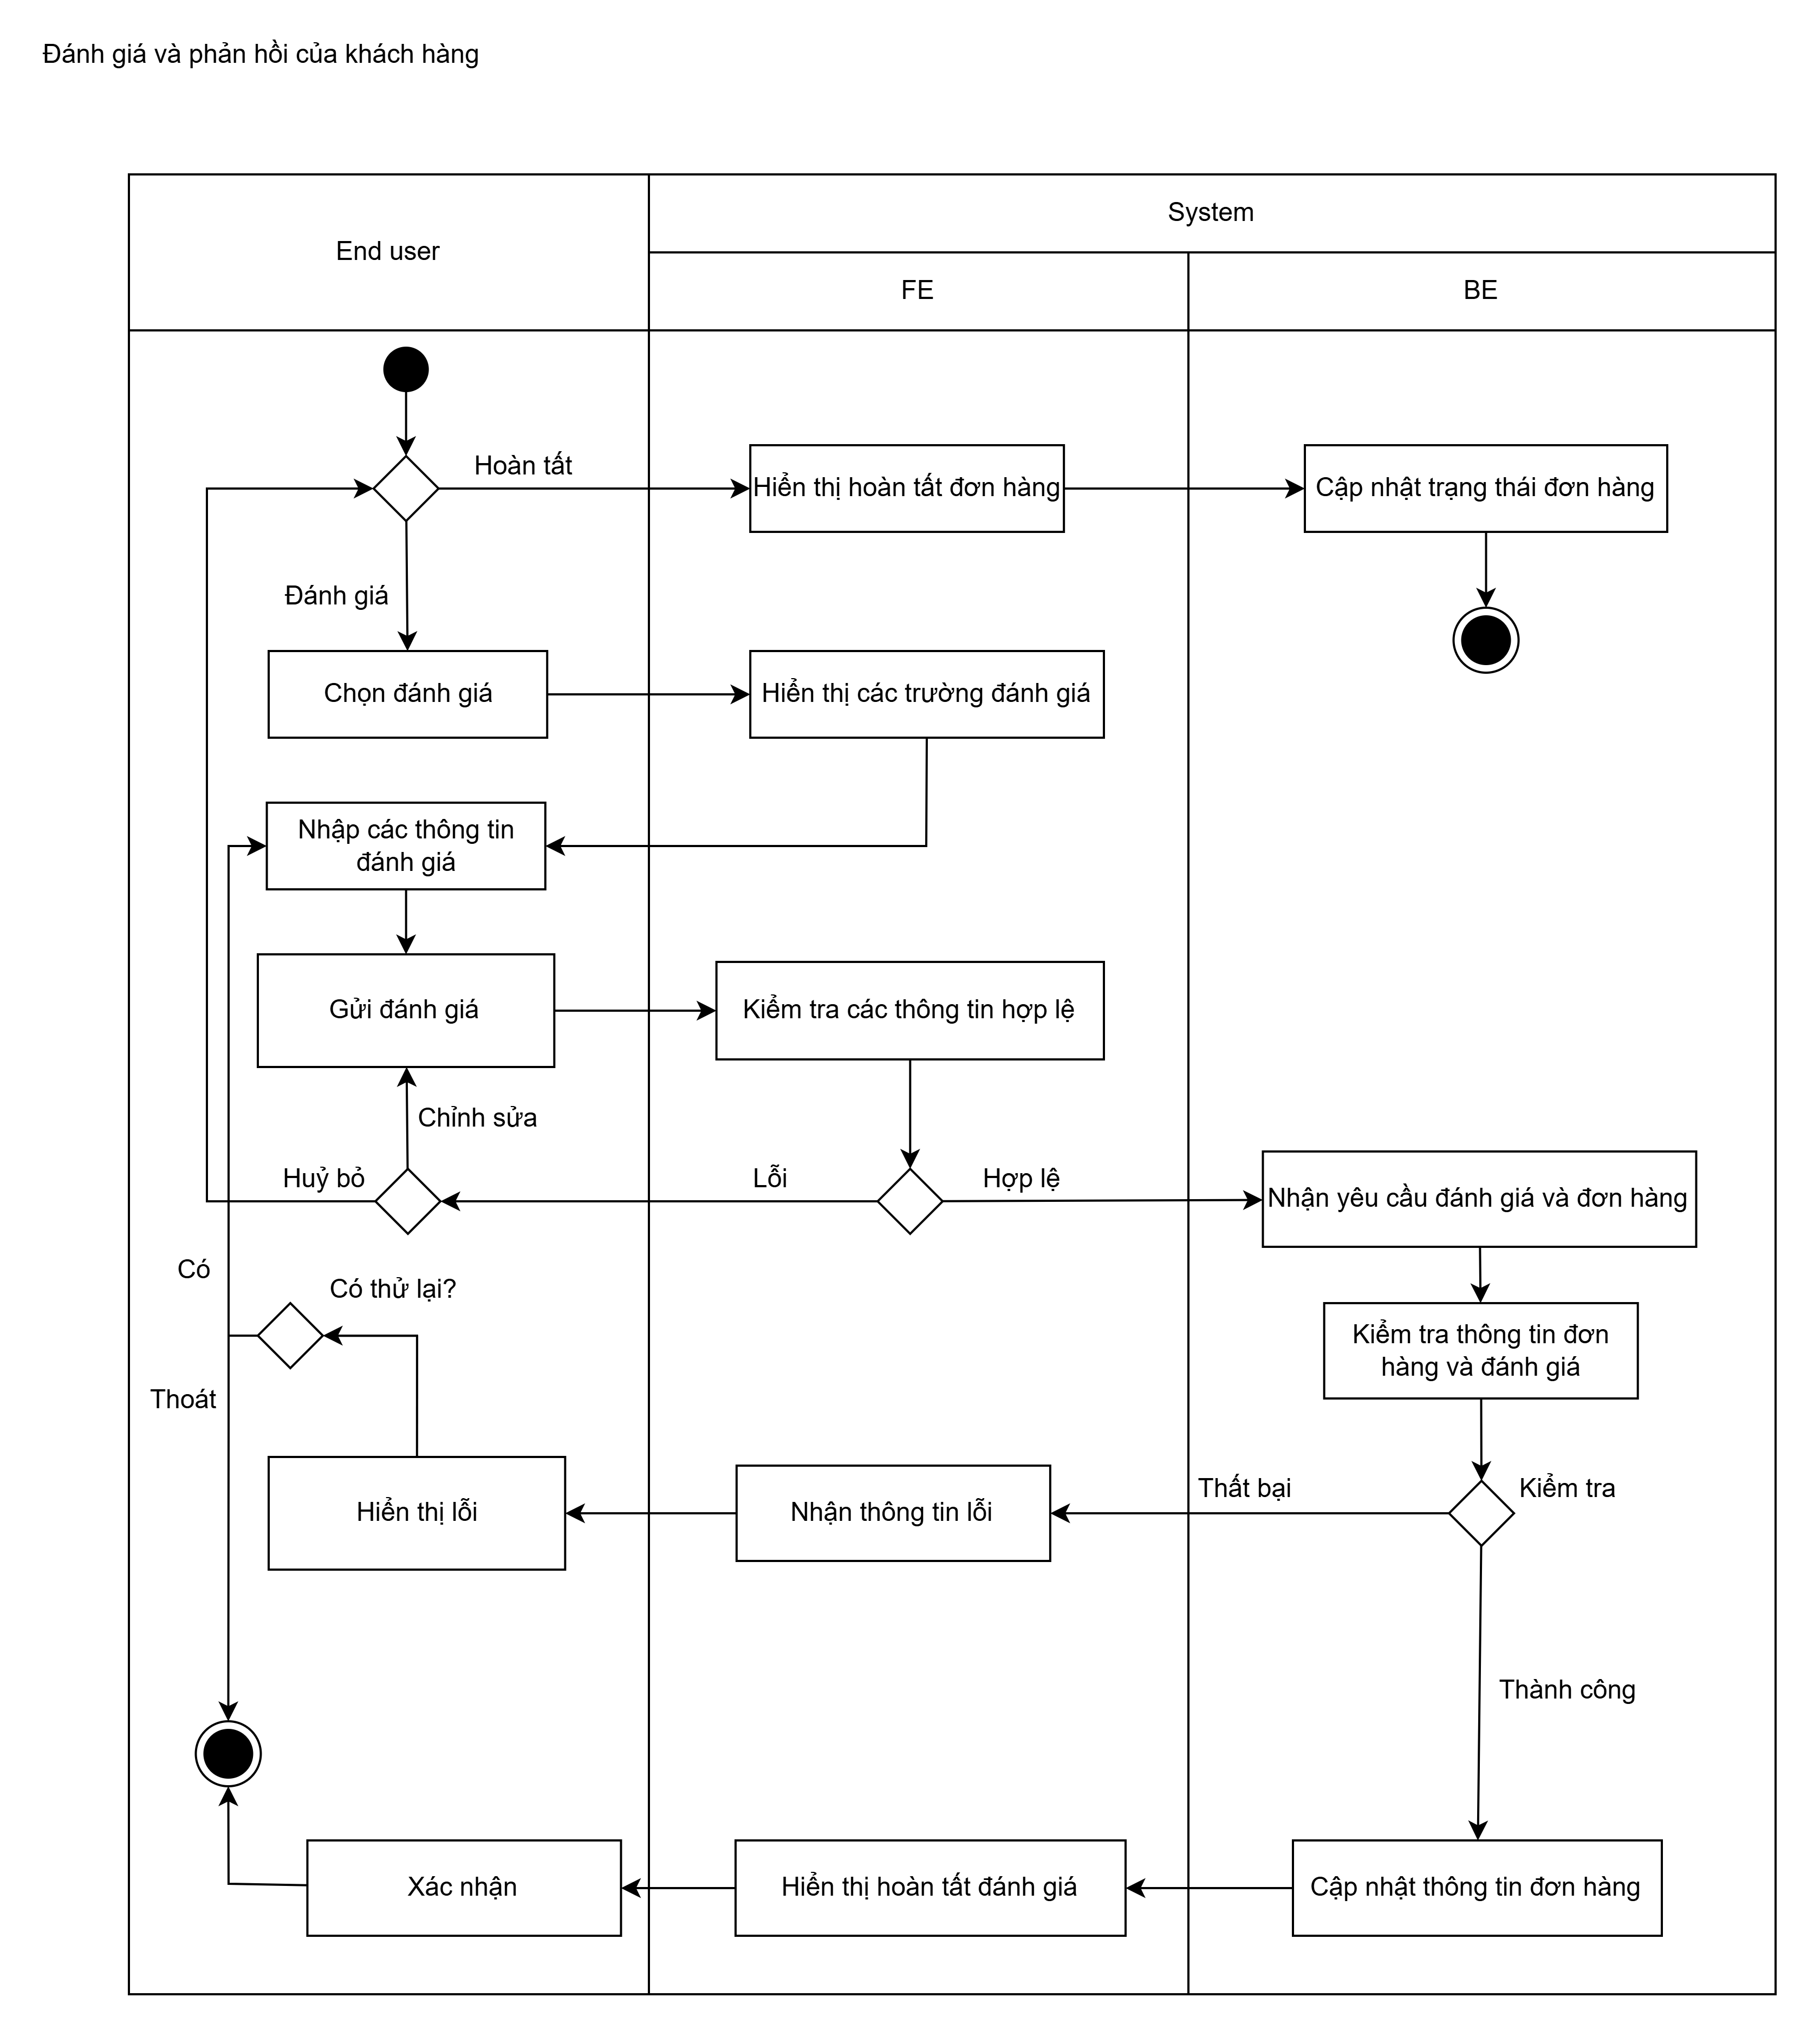
\includegraphics[width=0.7\linewidth]{images/chap3/activity_diagram/customer_feedback.png}
   \vspace{0.5cm} \caption{Sơ đồ hoạt động Phản hồi ý kiến khách hàng}
    \label{fig:act_feedback}
\end{figure}
Quy trình ghi nhận đánh giá, nhận xét của khách hàng về sản phẩm hoặc dịch vụ để cải thiện chất lượng hệ thống.

% --- PHẦN 5: QUẢN TRỊ VIÊN (ADMINISTRATION) ---

\begin{figure}[H]
    \centering
    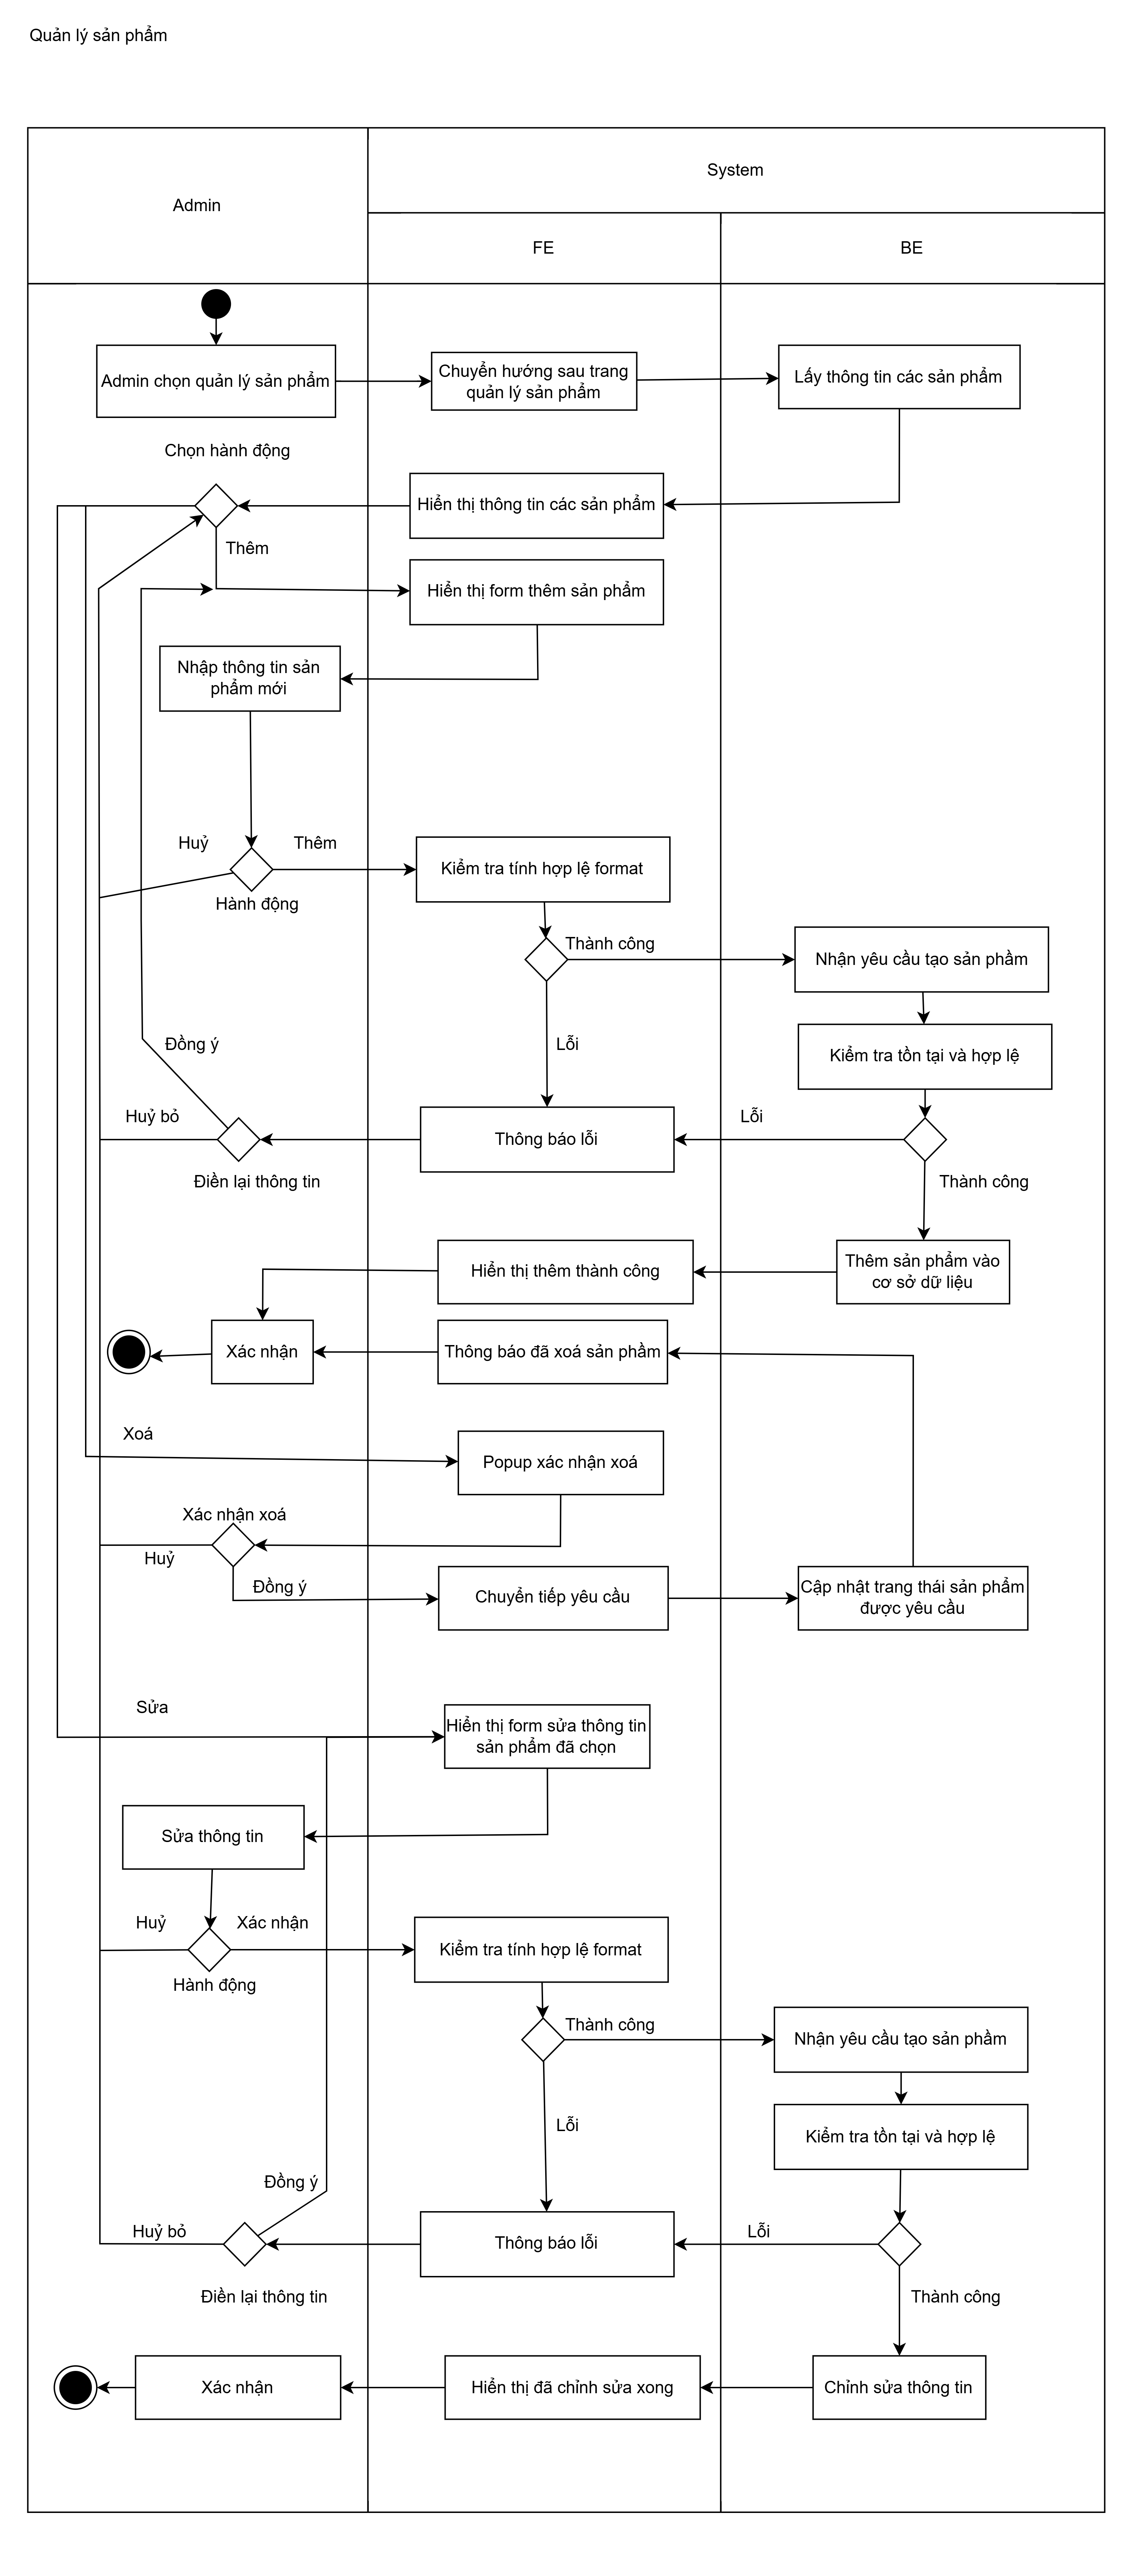
\includegraphics[width=0.6\linewidth]{images/chap3/activity_diagram/manage_product.png}
   \vspace{0.5cm} \caption{Sơ đồ hoạt động Quản lý sản phẩm (Admin)}
    \label{fig:act_manage_product}
\end{figure}
Dành cho Quản trị viên: Thực hiện các chức năng Thêm mới, Cập nhật thông tin, hoặc Ẩn/Xóa sản phẩm khỏi hệ thống.

\begin{figure}[H]
    \centering
    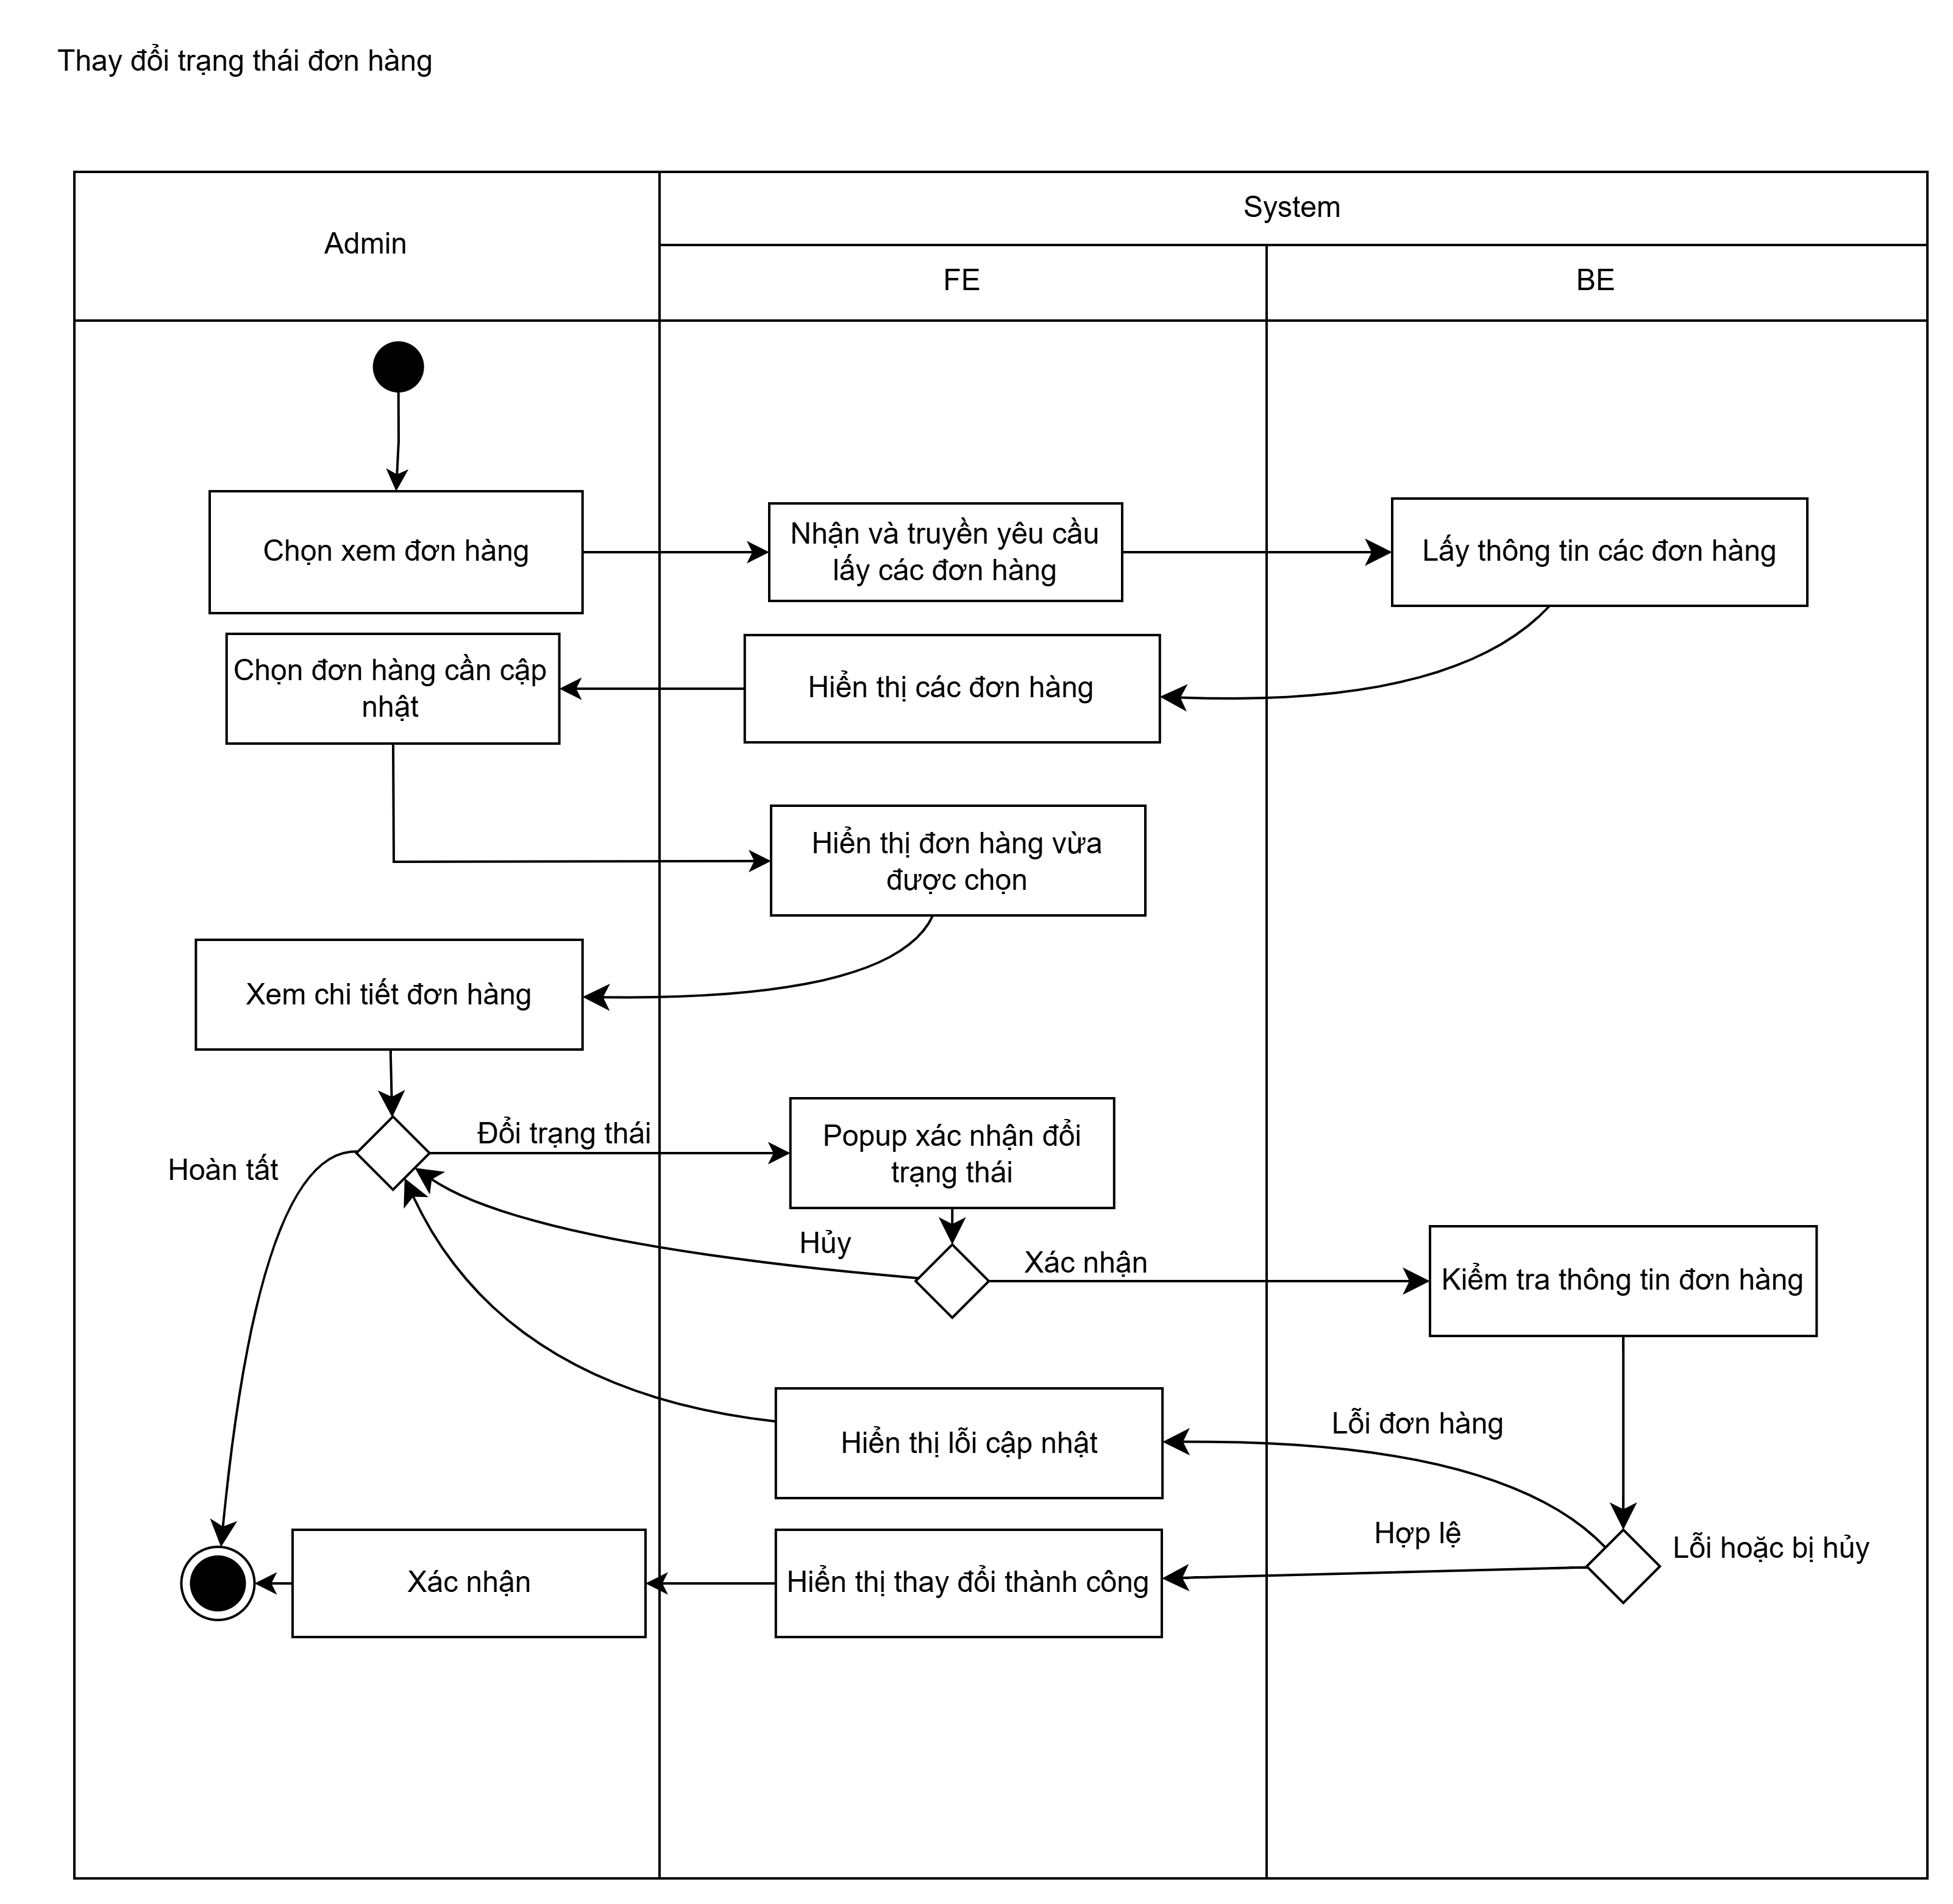
\includegraphics[width=0.8\linewidth]{images/chap3/activity_diagram/change_order_status.png}
   \vspace{0.5cm} \caption{Sơ đồ hoạt động Cập nhật trạng thái đơn hàng (Admin)}
    \label{fig:act_change_status}
\end{figure}
Quy trình xử lý đơn hàng phía Admin: Xác nhận đơn, chuyển sang trạng thái đóng gói, giao hàng, hoặc hoàn tất đơn hàng.

\begin{figure}[H]
    \centering
    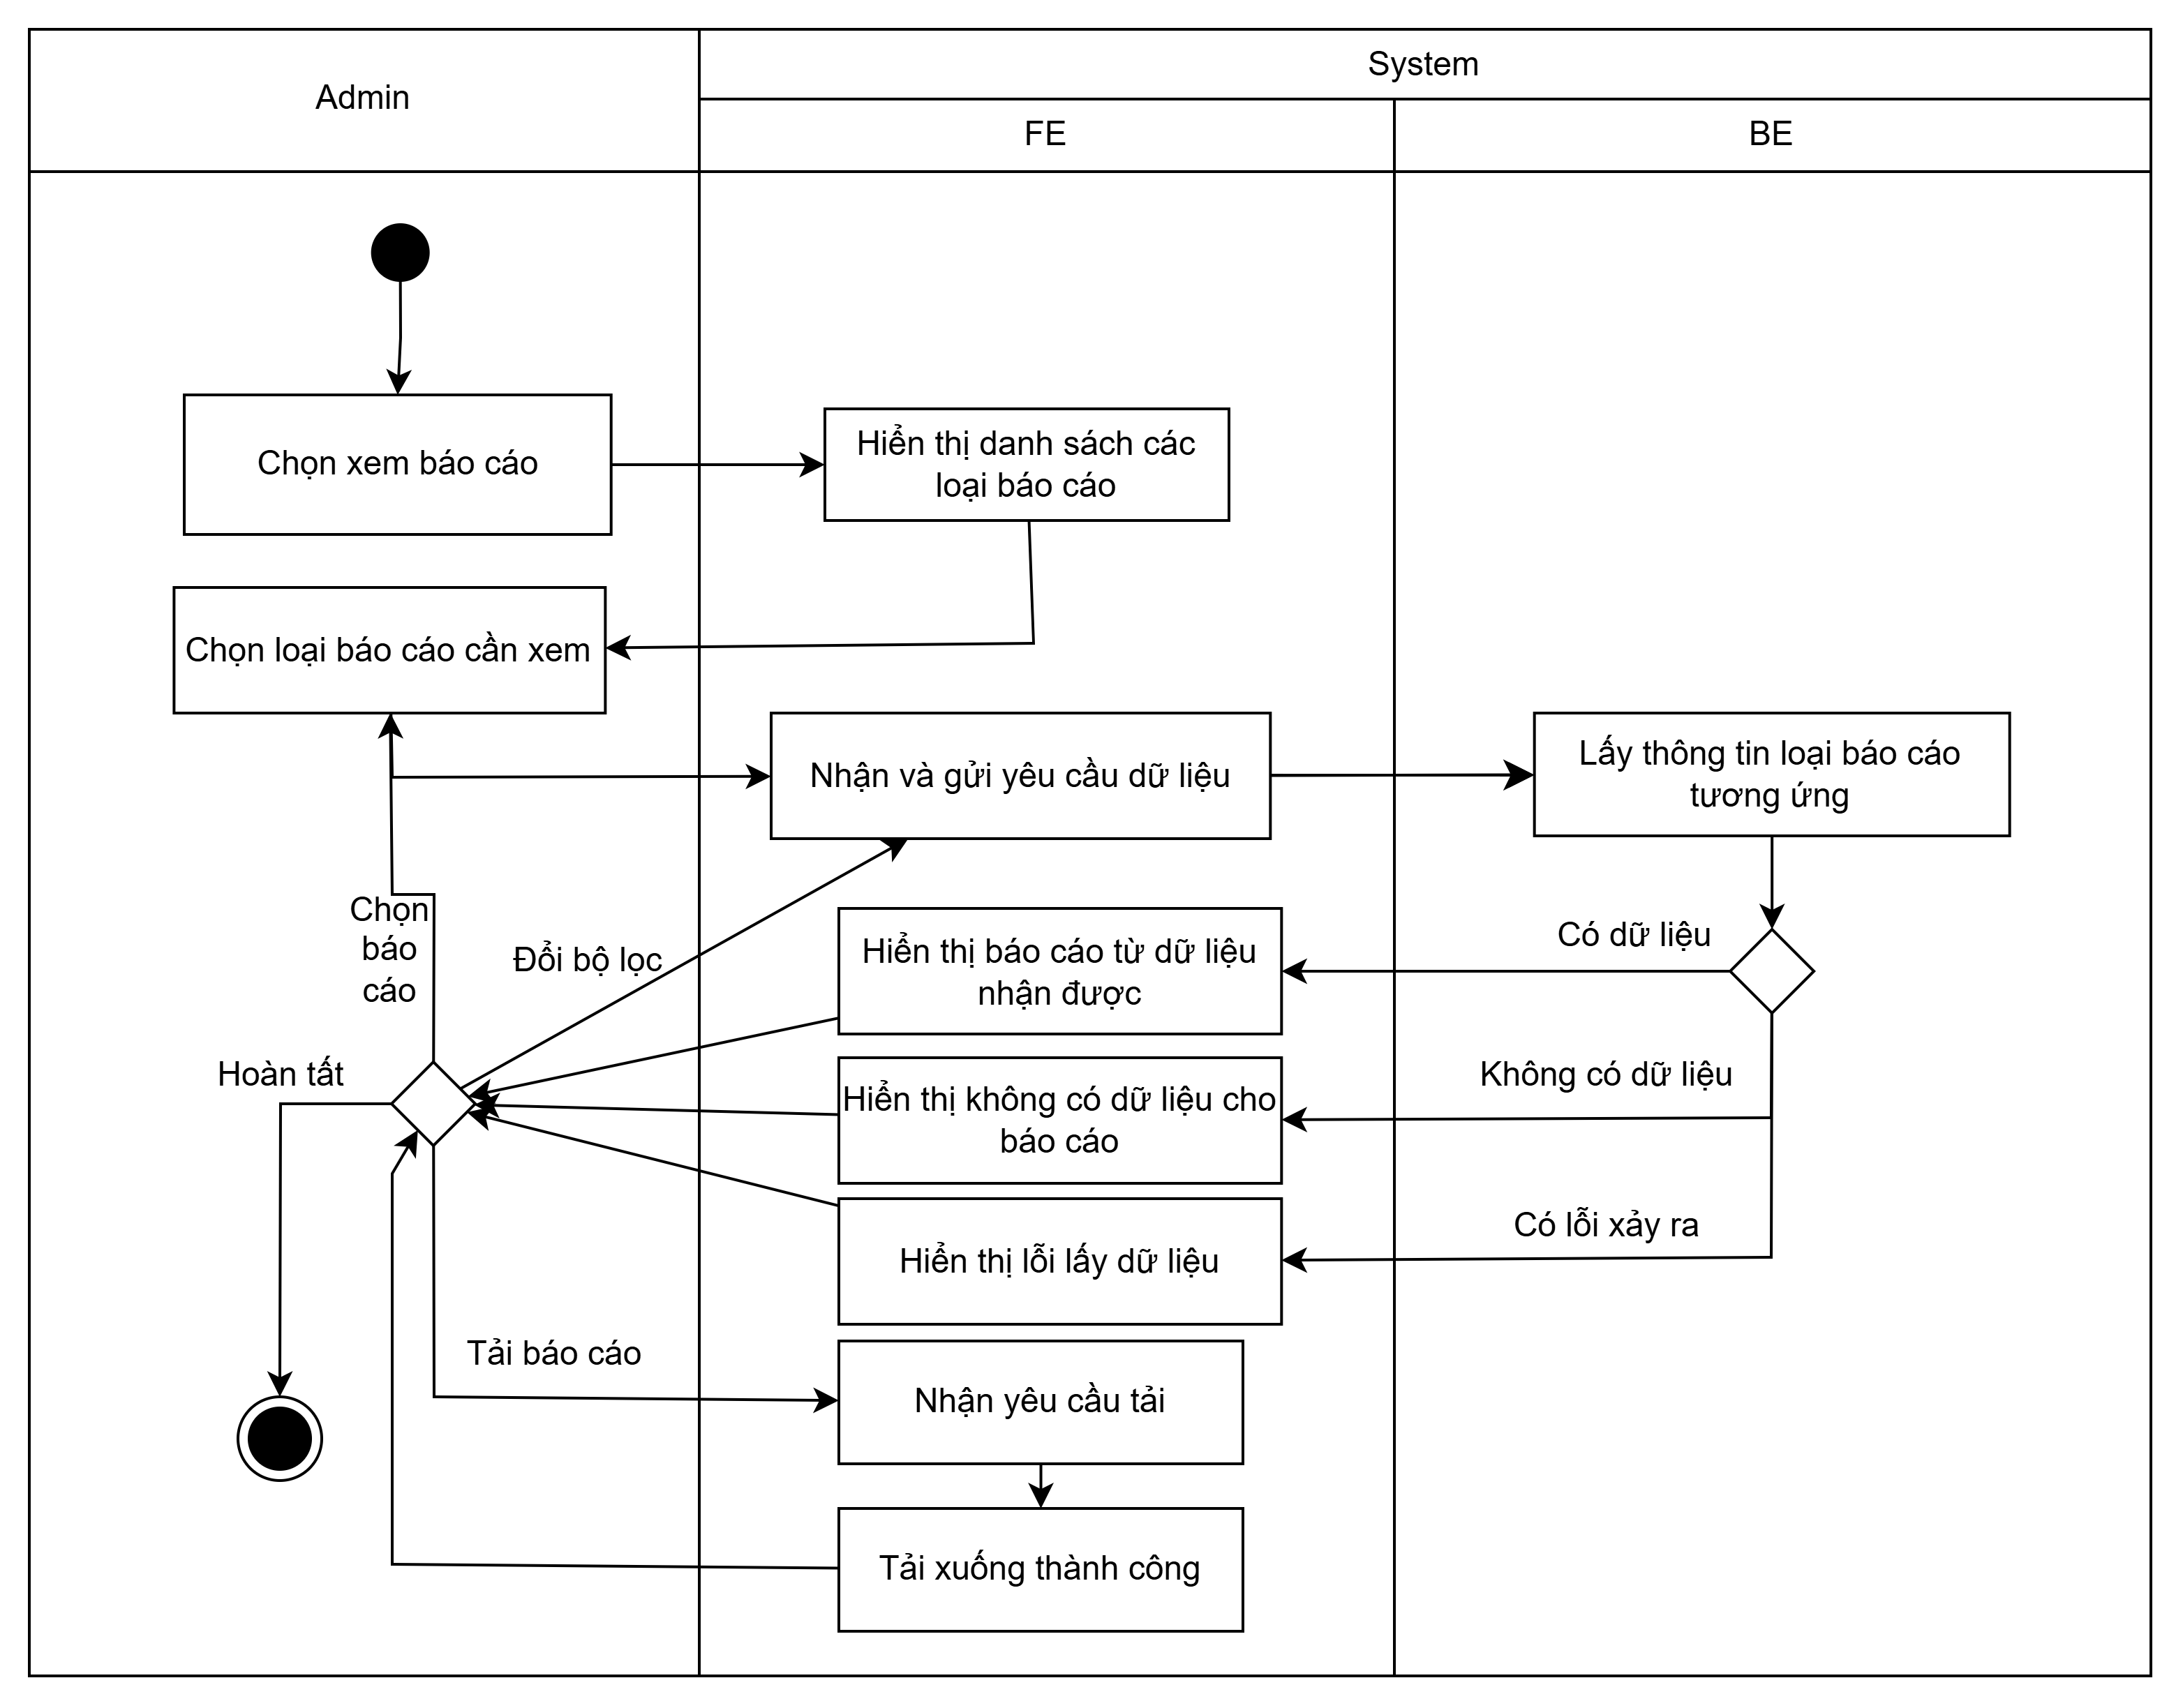
\includegraphics[width=0.8\linewidth]{images/chap3/activity_diagram/view_basic_report.png}
   \vspace{0.5cm} \caption{Sơ đồ hoạt động Xem báo cáo thống kê}
    \label{fig:act_report}
\end{figure}
Chức năng tổng hợp dữ liệu, hiển thị báo cáo doanh thu, số lượng đơn hàng và tồn kho cho người quản lý.